% !TeX program = pdflatex
% Диссертация по ГОСТ. Русский язык, кириллица, класс report для глав
\documentclass[12pt,a4paper]{report}

% Кодировки и русский язык
\usepackage[utf8]{inputenc}
\usepackage[T2A]{fontenc}
\usepackage[russian]{babel}

% Поля по ГОСТ (примерно: 30/10/20/20 мм). Настройте при необходимости
\usepackage{geometry}
\geometry{left=30mm,right=20mm,top=20mm,bottom=20mm}

% Межстрочный интервал 1.5
\usepackage{setspace}
\onehalfspacing

% Абзацный отступ и выравнивание
\usepackage{indentfirst}
\setlength{\parindent}{12.5mm}
\sloppy

% Математика
\usepackage{amsmath,amssymb,amsthm}
\numberwithin{equation}{chapter}

% Графика (на будущее)
\usepackage{graphicx}
\usepackage{float}
\usepackage{wrapfig}

% Содержание с точками
\usepackage{tocloft}
\renewcommand{\cftsecleader}{\cftdotfill{\cftdotsep}}

% Оформление подписей
\usepackage[labelsep=period]{caption}
\captionsetup{justification=centering}

% Список литературы с BibTeX
\usepackage[numbers,sort&compress]{natbib}
% Гиперссылки и поддержка \url в .bbl
\usepackage[unicode]{hyperref}
\bibliographystyle{unsrtnat}

% Команды для обозначений
\newcommand{\vect}[1]{\boldsymbol{#1}}
\newcommand{\tr}{\operatorname{tr}}

\begin{document}

% \thispagestyle{empty}
\begin{center}
\Large Наименование организации\\[10pt]
\large Диссертация\\[24pt]
\LARGE Математическое описание модели CLANN\\[6pt]
\Large (Convex Laplace Artificial Neural Network)\\[24pt]
\large Автор: Ф.И.О.\\[6pt]
Научный руководитель: Ф.И.О., уч. степень, звание\\[24pt]
Город — Год
\end{center}
\newpage




% \chapter*{Реферат}
Краткая характеристика работы, объём, иллюстрации, таблицы, источники. Основные результаты и новизна.
\addcontentsline{toc}{chapter}{Реферат}




% \chapter*{Условные обозначения, сокращения и термины}
CLANN — Convex Laplace Artificial Neural Network.\\
ICNN — Input Convex Neural Network.\\
ПК2 — Второй тензор Пиола—Кирхгофа.\\
SPD — Симметричный положительно определённый.\\
\addcontentsline{toc}{chapter}{Условные обозначения, сокращения и термины}




% \chapter*{Введение}
Актуальность, цель и задачи исследования, объект и предмет, научная новизна, практическая значимость, положения, выносимые на защиту, апробация, публикации, структура работы.
\addcontentsline{toc}{chapter}{Введение}




\tableofcontents
\newpage

% !TeX root = ../main_rus.tex
\chapter{Выпуклая нейронная сеть для основанной на данных симуляции гиперупругой механики с использованием меры деформации Лапласа (CLаNN)}

\section{Введение}

% Математические модели, способные предсказывать нелинейное механическое поведение мягких материалов при больших деформациях, требуются в широком спектре инженерных отраслей -- от полимерной промышленности, до робототехники и персонализированной медицины \cite{
% Mechanical characterization and FE modelling of a hyperelastic material
% Quantifying the uncertainty in a hyperelastic soft tissue model with stochastic parameters
% Control-oriented models for hyperelastic soft robots through differential geometry of curves
% }
% Основой таких моделей служит нелинейная теория упругости \cite{A Comparative Study of Several Material Models for Prediction of Hyperelastic Properties: Application to Silicone-Rubber and Soft Tissues}, где 
% зависимость тензора напряжений от переменных, характеризующих кинематику материала, описывается так называемыми определяющими соотношениями, или уравнениями состояния \cite{Nonlinear solid mechanics: a continuum approach for engineering science}. 
% При моделировании напряженно-деформированного состояния полимеров и биологических тканей широко распространены гиперупругие определяющие соотношения \cite{
% Hyperelastic structures: A review on the mechanics and biomechanics}.

% В гиперупругой постановке постулируется существование упругого потенциала $\psi$, зависящего от выбранной меры деформации, который полностью описывает механическое поведение материала. При этом он должен удовлетворять ряду требований: отражать материальную симметрию, не зависеть от выбранной системы отсчета, обладать свойствами поливыпуклости \cite{Convexity conditions and existence theorems in nonlinear elasticity}, что является достаточным условием существования решений краевых задач гиперупругости \cite{Mathematical elasticity: Three-dimensional elasticity
% Hyperelastic membrane modelling based on data-driven constitutive relations}.

% Для мягких материалов предложено множество гиперупругих моделей \cite{Hyperelastic energy densities for soft biological tissues: a review}, большинство из которых удовлетворяют требованиям к материальной симметрии, объективности и поливыпуклости благодаря инвариантному подходу. Это означает, что для выбранной меры деформации задается набор инвариантов, а упругий потенциал является функцией этих инвариантов. Обычной практикой является использование инвариантов правых/левых тензоров деформации Коши-Грина. Для изотропных материалов упругий потенциал может быть выражен как функция от трех инвариантов правого тензора деформации Коши-Грина $\psi = \psi_{vol}(J) + \psi_{iso}(I_1,I_2,I_3)$, где $J$ -- якобиан, выражающий изменение объема тела при деформации, $I_1, I_2, I_3$ -- инварианты правого тензора деформации Коши-Грина. 
% Дальнейшим расширением инвариантного подхода является введение так называемых псевдоинвариантов правого тензора Коши-Грина $I_4,...I_8$, позволяющих описывать классы трансверсально-изотропных и ортотропных материалов. \cite{Nonlinear solid mechanics: a continuum approach for engineering science}.
% %Для несжимаемого трансверсально-изотропного материала упругий потенциал задается как $\psi = \psi_{iso}(I_1,I_2,I_3) + \psi_{aniso}(I_4,I_5)$ .
% %, где $I_4 = \mathbf{a_0} (\mathbf{F}^{\mathrm{T}} \mathbf{F})\mathbf{a_0}$, $I_5 = \mathbf{a_0} (\mathbf{F}^{\mathrm{T}} \mathbf{F})^2 \mathbf{a_0}$ 
% Такой подход требует априорного задания упругого потенциала аналитической функцией с параметрами, которые определяются из экспериментальных данных. Основными недостатками этого подхода являются неединственность оптимального набора параметров модели, отсутствие у инвариантов прямого физического смысла в терминах деформации \cite{On the use of the upper triangular (or QR) decomposition for developing constitutive equations for Green-elastic materials} с вытекающим из этого требованием к натурному эксперименту, а именно, достижение однородности деформаций и напряжений при механическом исследовании тестировании материала, субъективность выбора формы потенциала из множества построенных экспертами моделей \cite{Interpretable data-driven modeling of hyperelastic membranes}.

% В некоторой степени, эти недостатки устраняют конструированием наилучшей гиперупругой модели регрессионными методами из набора априорно заданных мономов на основе инвариантов \cite{A new family of Constitutive Artificial Neural Networks towards automated model discovery}, или редукцией обобщенных моделей на основе информационного анализа экспериментальных данных \cite{On the AIC-based model reduction for the general Holzapfel–Ogden myocardial constitutive law}. В совокупности с полнополевыми методами оценки экспериментальных деформаций (цифровая корреляция избражений DIC \cite{High-speed 3D digital image correlation vibration measurement: Recent advancements and noted limitations}), методами виртуальных полей VFM \cite{VFM} и inverse FE \cite{NN-Euclid}, это становится мощным инструментом моделирования механики материалов в рамках гиперупругости. Однако, такие подходы остаются феноменологическими и все так же требуют экспертный выбор модели.

% Важное преимущество гиперупругой постановки состоит в том, что она не требует знания аналитического вида упругого потенциала. Для задания определяющих соотношений в случае гиперупругого материала, достаточно знать производные упругого потенциала по выбранной мере деформации, так называемые функции отклика \cite{Nonlinear solid mechanics: a continuum approach for engineering science}. С применением полнополевых методов оценки экспериментальных деформаций DIC и напряжений \cite{Numerical_study_of_stress_estimation_methods_for_membrane_inflation
% In vitro analysis of localized aneurysm rupture}, функции отклика могут быть построены напрямую на основе экспериментальных данных, полученных при тестировании материала в широком диапазоне различных режимов деформации. Это стимулирует исследование подходов к построению гиперупругих моделей, основанных на данных \cite{Data-driven computational mechanics}. 

% В работах \cite{Interpretable data-driven modeling of hyperelastic membranes
% Data-Driven Anisotropic Biomembrane Simulation Based on the Laplace Stretch} предлагается метод прямого моделирования механики изотропных и анизотропных материалов, основанного на данных, с использованием функций отклика, основанных на физически интерпретируемой мере деформации Лапласа\cite{On the use of the upper triangular (or QR) decomposition for developing constitutive equations for Green-elastic materials
% Laplace stretch: Eulerian and Lagrangian formulations}, в котором обходят проблемы инвариантной формулировки гиперупругой модели, напрямую строя функции отклика на основе экспериментальных данных. При этом не требуются какие-либо предварительные знания о симметрии материала. Совокупность функций отклика формирует таблично-заданное определяющее соотношение.
% Нелинейная система алгебраических уравнений для виртуального квазистатического растяжения и раздутия материалов в этих случаях решается простым методом релаксации, где метод интерполяции обратного взвешенного расстояния находит требуемые значения функций отклика на каждой итерации в любой точке пространства деформаций Лапласа. 
% Ограничениями такого подхода являются требования к "богатству" данных и невозможность применения градиентных методов решения нелинейных систем алгебраических уравнений в силу дискретности таблично-заданного определяющего соотношения.

% Параллельно с этим развиваются физически-информированные нейросетевые подходы, в частности выпуклые по входу нейронные сети (ICNN) \cite{Input Convex Neural Networks}, позволяющие "вшивать" в архитектуру сети объективность, монотонность и выпуклость по входу, являясь прокси к поливыпуклости, тем самым удовлетворяя требованиям к гиперупругим потенциалам \cite{Benchmarking physics-informed frameworks for data-driven hyperelasticity}. В работе \cite{NEURAL NETWORKS MEET ANISOTROPIC HYPERELASTICITY: A FRAMEWORK BASED ON GENERALIZED STRUCTURE TENSORS AND ISOTROPIC TENSOR FUNCTIONS} показана инвариантная архитектура физически-информированной нейронной сети, совместимая с конечно-элементными пакетами. Несмотря на интерпретируемость и термодинамическую корректность, архитектура сети включает в себя набор предположений -- обобщенных структурных тензоров \cite{Ebbing Phd}, что фактически фиксирует класс симметрии материала.

% В рамках данной работы мы предлагаем подход, который объединяет преимущества представления гиперупругой модели таблично-заданным определяющим соотношением в мерах деформаций Лапласа \cite{Data-Driven Anisotropic Biomembrane Simulation Based on the Laplace Stretch} и физически-информированных нейронных сетей \cite{Input Convex Neural Networks}, удовлетворяющих требованиям к гиперупругим моделям механики материалов. Мы формулируем термодинамически корректный, объективный по построению, выпуклый по входу, и не требующий знаний о симметрии материала гиперупругий потенциал, в котором анизотропия восстанавливается непосредственно из данных. Гладкость аппроксимации обеспечивает совместимость с градиентными методами решения систем нелинейных алгебраических уравнений. В сравнении с таблично-заданными определяющими соотношениями, CLaNN снимает ограничения, связанные с дискретностью аппроксимации, сохраняя интерпретируемость мер деформации и повышая устойчивость экстраполяции.

\paragraph{Область применимости и ограничения}
квазистатика, мембранная постановка...

\paragraph{Организация статьи}

\section{Кинематика}
\textbf{Основные соотношения}

Мы рассматриваем равновесие тонкой несжимаемой гиперупругой мембраны с толщиной $H$ под
определенными нагрузками.
Деформация мембраны характеризуется деформацией её срединной поверхности. 
Обозначим через \(\mathbf{X}\) и \(\mathbf{x}\) положения точек, 
в соответствующих базисах \(\vect{E}_{\alpha}\) и \(\vect{e}_{\alpha}\), 
в исходной (недеформированной) \(\Omega_0 \subset \mathbb{R}^2\) и текущей (деформированной) \(\Omega_t \subset \mathbb{R}^2\)
конфигурациях поверхности мембраны соответственно. 
Деформация определяется отображением \(\mathbf{x} = \mathbf{x}(\mathbf{X})\), 
поверхностный градиент деформации \(\mathbf{F} = \vect{e}_{\alpha} \otimes \vect{E}^{\alpha}\),
а правый тензор Коши—Грина \(\vect C = C_{\alpha\beta} \;\vect{e}_{\alpha} \otimes \vect{e}_{\beta} = \vect F^{\top} \vect F\). 
Для определения меры деформации мы используем меру Лапласа \(\vect{\xi} = (\xi_1 , \xi_2 , \xi_3)^T\) \cite{xi2023},
которая может быть вычислена двумя эквивалентными способами: 
либо через QR-разложение градиента деформации \(\vect F = \vect Q \vect R\) с \(\vect U = \vect R\) , 
либо через разложение Холецкого правого тензора Коши-Грина \(\vect C = \vect U^{\top}\vect U\) (Приложение \ref{app:cholesky}).
В этом случае гиперупругий потенциал является функцией от деформации Лапласа \(\psi = \psi(\vect{\xi})\).


\textbf{Мера деформации Лапласа}
В двумерном случае вводятся характеристики
\begin{equation}
\xi_1 = \ln(u_{11}),\quad \xi_2 = \ln(u_{22}),\quad \xi_3 = \frac{u_{12}}{u_{11}}, 
\quad \vect{U} = u_{\alpha\beta} \; \vect{e}_{\alpha} \otimes \vect{e}_{\beta}.
\label{eq:laplace_coords}
\end{equation}



\section{Напряжение и термодинамическая корректность}
\textbf{Второй тензор напряжений Пиолы-Кирхгофа} вычисляется по цепному правилу дифференцированием энергии \(\psi\) 
по правому тензору деформации Коши-Грина \(\vect C\):

\begin{equation}
  \mathbf{S} \;=\; 2\,\frac{\partial \psi}{\partial \mathbf{C}}
  \;=\; 2\,\frac{\partial \psi}{\partial \boldsymbol\xi} \cdot \frac{\partial \boldsymbol\xi}{\partial \mathbf{C}}
  \;=\; 2\,\mathbf{r}(\boldsymbol\xi)\cdot\frac{\partial \boldsymbol\xi}{\partial \mathbf{C}},
  \qquad \mathbf{r}:=\frac{\partial \psi}{\partial \boldsymbol\xi}.
  \label{eq:chain-rule}
\end{equation}

Такое построение имеет ключевые следствия:
\begin{itemize}
  \item \textbf{Объективность:} $\psi(\mathbf{C})=\psi(\mathbf{Q}^\top\mathbf{C}\mathbf{Q})$ для любой ортогональной $\mathbf{Q}$, а значит и $\mathbf{S}$ инвариантен к поворотам.
  \item \textbf{Симметрия напряжений:} $\mathbf{S}=\mathbf{S}^\top$ вследствие симметрии $\mathbf{C}$ и корректного применения цепного правила.
  \item \textbf{Термодинамическая корректность:} равенство \eqref{eq:chain-rule} является следствием неравенства Клаузиуса-Дюгема 
  $\mathcal{D} = \mathbf{S} : \dot{\mathbf{C}} - \dot{\psi}(\mathbf{C}) \geq 0$, 
  выражающее второе начало термодинамики для механических процессов \cite{truesdell1984historical,truesdell2004nonlinear}.
\end{itemize}

\textbf{Связь тензора Лапласа и второго тензора напряжений Пиолы-Кирхгофа}

Применяя цепное правило дифференцирования к выражению \eqref{eq:chain-rule} и используя меру деформации Лапласа, 
получаем аналитические выражения для компонент второго тензора напряжений Пиолы-Кирхгофа в двумерном случае:

\begin{equation}
\begin{aligned}
  S_{11} &= e^{-2\xi_1}\big(r_1-2\xi_3 r_3\big) + e^{-2\xi_2} r_2\,\xi_3^2,\\
  S_{22} &= e^{-2\xi_2} r_2,\\
  S_{12} &= -e^{-2\xi_2} r_2\,\xi_3 + e^{-2\xi_1} r_3,
\end{aligned}
\label{eq:stress_components_2d}
\end{equation}
$r_1, r_2, r_3$ — компоненты функции отклика $\mathbf{r} = \frac{\partial \psi}{\partial \boldsymbol\xi}$.

% Эти соотношения демонстрируют связь между логарифмическими мерами деформации и компонентами напряжений, 
% характерную для гиперупругих материалов. 
% Экспоненциальные множители $e^{-2\xi_i}$ отражают логарифмическую природу выбранной параметризации, 
% а члены, содержащие $\xi_3$, описывают сдвиговые эффекты.

\textbf{Фундаментальные ограничения}

В соответствии с принципами термодинамики и механики сплошных сред, 
гиперупругая модель должна удовлетворять ряду фундаментальных ограничений, обеспечивающих физическую корректность и 
материальную устойчивость.
\begin{enumerate}
  \item \textbf{Неотрицательность.}
  \begin{equation}
    \psi(\vect{\xi}) \ge 0\quad \forall\,\vect{\xi}\in\mathbb{R}^3.
  \end{equation}
  Это исключает отрицательную внутреннюю энергию и согласуется с трактовкой потенциальной энергии как накопленной работы упругих сил.
  \item \textbf{Нулевые значения для $\psi$ и $\vect S$ в естественном состоянии.}
  \begin{equation}
    \psi(\vect 0)=0,\qquad \vect S(\vect I)=\vect 0,
    \label{eq:natural_state_stress}
  \end{equation}
  Естественная (недеформированная) конфигурация является энергетическим минимумом и не порождает остаточных напряжений.
  \item \textbf{Бесконечный рост (коэрцитивность).}
  \begin{equation}
    \psi(\vect{\xi}) \to \infty\ \text{при}\ \lVert\vect{\xi}\rVert\to\infty,\qquad
    \vect{S} \to \infty\ \text{при}\ J\to\infty \text{ или } J\to 0^{+},\qquad
    J=\det\vect F,
    \label{eq:energy_constraints}
  \end{equation}
  Это обеспечивает коэрцивность: крайние объёмные деформации ($J\to\infty$, $J\to 0^{+}$) и неограниченный рост меры деформации физически недостижимы при конечной работе.
\end{enumerate}

Эти свойства принято записывать через градиент деформации $\vect{F}$ и правый тензор деформации Коши-Грина $\vect{C}$ 
\cite{antman2005nonlin,green1839laws,kirchhoff1850gleichgewicht}, но они эквивалентны и для меры деформации Лапласа $\vect{\xi}$.


\section{Архитектура CLaNN и её производные}


В рамках предложенного под  хода CLaNN (Convex Laplace Neural Network)
энергия деформации \(\psi(\vect{\xi})\) с мерой деформации Лапласа аппроксимириуется посредством 
выпуклой по входу нейронной сетью (Input Convex Neural Network, ICNN) \cite{icnn2017}
и вычисления 2 тензора напряжения Пиолы-Кирхгофа \(\vect{S}\). 

\textbf{Обобщенная архитектура ICNN}

ICNN представляет собой класс нейронных сетей, гарантирующих выпуклость выходной функции относительно входных переменных. 
В нашем случае, функция энергии деформации $\psi: \mathbb{R}^3 \rightarrow \mathbb{R}$ называется выпуклой, 
если $\forall \vect{\xi}_1, \vect{\xi}_2 \in \mathbb{R}^3$ и $\lambda \in [0,1]$ выполняется неравенство Йенсена:
\begin{equation}
\psi(\lambda \vect{\xi}_1 + (1-\lambda) \vect{\xi}_2) \leq \lambda \psi(\vect{\xi}_1) + (1-\lambda) \psi(\vect{\xi}_2).
\label{eq:convexity_definition}
\end{equation}

Ключевые условия ICNN \cite{icnn2017}: 
(i) поэлементно выпуклая, монотонно неубывающая активация $\varphi$; 
(ii) $\mathbf{W}_z^{(\ell)}\!\ge\!0$ для всех слоёв 
(только на связях $z\!\to\!z$; $\mathbf{W}_x^{(\ell)}$, $\mathbf{b}^{(\ell)}$ без ограничений по знаку); 
(iii) каждый слой имеет прямую аффинную связь с входом 
$\boldsymbol{\xi}$: $z^{(\ell+1)}=\varphi\!\big(\mathbf{W}_z^{(\ell)}z^{(\ell)}+\mathbf{W}_x^{(\ell)}\boldsymbol{\xi}+\mathbf{b}^{(\ell)}\big)$; 
(iv) скалярный выход как $a^{\top} z^{(L)}+c$ с $a\!\ge\!0$ (или ещё один слой $\varphi$).

\textbf{Шаг 1. Однослойный ICNN и выбор активации.}
Рассмотрим однослойный вариант ICNN (с одним скрытым слоем) для аппроксимации $\psi(\boldsymbol{\xi})$:
\begin{equation}
  s = \mathbf{W}_1 \,\boldsymbol{\xi} + \mathbf{b}_1,\qquad
  z = \varphi_{\beta}(s),\qquad
  \tilde{\psi} = \mathbf{W}_2^{\top} z + b_2,\qquad \mathbf{W}_2 \ge 0.
  \label{eq:icnn_onelayer}
\end{equation}

\begin{equation}
  \varphi_{\beta}(x) = \frac{\operatorname{softplus}(\beta x)}{\beta},
  \label{eq:softplus_activation}
\end{equation}

Здесь $\varphi_{\beta}$ — выпуклая неубывающая функция активации \cite{dugas2001incorporating}, 
которая гладко аппроксимирует ReLU и при конечных $\beta$ является строго выпуклой; $\varphi_{\infty}(x)=\max(0,x)$.
Условие $\mathbf{W}_2\!\ge 0$ сохраняет выпуклость линейной комбинации. 
Размерности: $\mathbf{W}_1\!\in\mathbb{R}^{h\times 3}$, $\mathbf{b}_1\!\in\mathbb{R}^{h}$, 
$\mathbf{W}_2\!\in\mathbb{R}^{h}_{\ge 0}$, $h$ — размерность скрытого слоя.

\textbf{Шаг 2. Центрирование энергии $\psi$ в естественном состоянии.}
Для выполнения условия $\psi(\mathbf{0})=0$ центрируем энергию, 
вычитая значение нелинейной части при $\boldsymbol{\xi}=\mathbf{0}$:
\begin{equation}
  z_0 = \varphi_{\beta}(\mathbf{b}_1),\qquad
  \psi(\boldsymbol{\xi}) = \mathbf{W}_2^{\top}\big(z - z_0\big),\qquad (b_2 \equiv 0).
  \label{eq:center_psi}
\end{equation}
Тогда $\psi(\mathbf{0})=0$. Поскольку $z_0$ не зависит от $\boldsymbol{\xi}$, 
градиент $\partial\psi/\partial\boldsymbol{\xi}$ и гессиан $\partial^2\psi/\partial\boldsymbol{\xi}^2$ 
совпадают с таковыми для $\tilde{\psi}$, сохраняя выпуклость и гладкость.

\textbf{Шаг 3. Центрирование отклика $\mathbf{r}$ в естественной конфигурации.}
Для выполнения условия $\vect S(\vect I)=\vect 0$ обнулим линейный отклик в точке 
$\boldsymbol{\xi}=\mathbf{0}$:
\begin{equation}
  \mathbf{r}_0 := \frac{\partial \psi}{\partial \boldsymbol{\xi}}\bigg|_{\boldsymbol{\xi}=\mathbf{0}},\qquad
  \psi_{\mathrm{phys}}(\boldsymbol{\xi}) = \psi(\boldsymbol{\xi}) - \mathbf{r}_0^{\top}\boldsymbol{\xi}.
  \label{eq:phys_energy}
\end{equation}

Тогда $\psi_{\mathrm{phys}}(\mathbf{0})=0$ и $\mathbf{r}(\mathbf{0})=\mathbf{0}$, 
а по цепному правилу \eqref{eq:chain-rule} получаем $\mathbf{S}(\mathbf{I})=\mathbf{0}$. 
Вычитание линейного члена не меняет гессиан и сохраняет выпуклость. 
Так как $\mathbf{r}(\mathbf{0})=\mathbf{0}$, точка $\boldsymbol{\xi}=\mathbf{0}$ является минимумом 
$\psi_{\mathrm{phys}}$, и значит $\psi_{\mathrm{phys}}\ge 0$.

После получения $\psi_{\mathrm{phys}}$ автоматически вычисляются 
$\partial\psi/\partial\boldsymbol{\xi}$ средствами autodiff, реализованными в современных библиотеках для машинного обучения 
\cite{pytorch2019}, \cite{tensorflow2016}, \cite{jax2018}, 
после чего тензор напряжений $\mathbf{S}$ находится по формуле \eqref{eq:stress_components_2d} с 
использованием связи $\psi(\vect C)=\psi\big(\boldsymbol{\xi}(\vect C)\big)$.

Центрирование $\psi_{\mathrm{phys}}$ и $\mathbf{r}$ в естественном состоянии 
дает возможность гарантирования выполнения \eqref{eq:natural_state_stress} и
позволяет избежать дополнительных ограничений на параметры сети


% Выбор функции активации $\operatorname{softplus}(\beta x)/\beta$ обусловлен её строгой выпуклостью и свойством $\lim_{\beta \to \infty} \operatorname{softplus}(\beta x)/\beta = \max(0,x)$, что обеспечивает плавный переход к функции ReLU при больших значениях параметра $\beta$. Ограничение $\vect W_2\ge 0$ является ключевым для сохранения выпуклости композиции функций, поскольку линейная комбинация выпуклых функций с неотрицательными коэффициентами остаётся выпуклой.



% (заменено на TikZ-схему в рис.~\ref{fig:clann_arc})

\textbf{Аналитические выражения для производных энергии}

\textbf{Градиент энергии деформации}

Аналитическое дифференцирование функции энергии по переменным \(\xi\) даёт выражение для градиента:

\begin{equation}
 \vect{r} = \nabla_\xi \psi_{\mathrm{phys}} = \vect W_1^T \left( \vect W_2 \odot \sigma(\beta (\vect W_1 \vect \xi + \vect b_1)) \right) - \vect r_0,
\label{eq:energy_gradient}
\end{equation}
где $\sigma(x) = \frac{1}{1 + e^{-x}}$ - сигмоида, 
а операция $\odot$ обозначает поэлементное произведение (Hadamard product). 
Данное выражение демонстрирует, что градиент энергии является линейной комбинацией строк матрицы $\vect W_1^T$ с весами, 
определяемыми произведением выходных весов $\vect W_2$ и значений функции активации $\sigma(\beta (\vect W_1 \vect\xi + \vect b_1))$.

\textbf{Гессиан энергии деформации}

Вторые производные энергии по переменным \(\xi\) определяют гессиан, который имеет следующую аналитическую форму:

\begin{equation}
 H_{ij} = \sum_h \sigma'_h\,W_{2,h}\,W_{h,i}W_{h,j},
\label{eq:energy_hessian}
\end{equation}

где $\sigma' = \beta\,\sigma(1-\sigma)$ - производная сигмоиды, 
$\sigma=\operatorname{sigmoid}(\beta s)$, а $s=\vect W_1\xi+\vect b_1$.

\textbf{Материальная устойчивость и положительная определённость}

% Строгая выпуклость функции энергии \(\psi(\xi)\) по переменным \(\xi\)
% имеет фундаментальное значение для материальной устойчивости гиперупругого материала. 
% Как показано в классических работах Болла (Ball, 1977) и Чиарлета (Ciarlet, 1988), 
% выпуклость энергии деформации является необходимым и достаточным условием для существования и единственности решения 
% задачи равновесия в нелинейной теории упругости.

Из строгой выпуклости \(\psi(\xi)\) следует положительная определённость гессиана:
\begin{equation}
 \vect H = \frac{\partial^2\psi}{\partial\xi^2} > 0,
\label{eq:positive_hessian}
\end{equation}
что обеспечивает положительную определённость касательных модулей упругости 
$\mathbb{C} = \partial^2\psi/\partial\vect C^2$ через цепное правило дифференцирования. 
Это свойство важно для численной стабильности конечно-элементных расчётов, 
поскольку на практике улучшает сходимость метода Ньютона и отсутствие сингулярностей в матрице жёсткости.


В рамках предложенного подхода обучение модели осуществляется путём минимизации функции потерь, 
которая количественно характеризует невязку между предсказанными и экспериментальными значениями напряжений:

\begin{equation}
 L = \frac{1}{N}\sum_{i=1}^N \lVert \vect S^{(i)}_{\text{pred}} - \vect S^{(i)}_{\text{exp}} \rVert^2.
\label{eq:main_loss_function}
\end{equation}

Для минимизации функции потерь \eqref{eq:main_loss_function} используется оптимизатор Adam \cite{kingma2014adam}, 
который широко используется в задачах машинного обучения. 
Процесс оптимизации включает вычисление градиентов по всем параметрам сети и обновление весов 
с использованием адаптивных моментов первого и второго порядка.

\begin{figure}[H]
  \centering
  \resizebox{\textwidth}{!}{% ===== CLaNN: однослойная ICNN (наглядная архитектура) =====
\begin{tikzpicture}[
  font=\small, node distance=9mm and 14mm, >={Latex},
  box/.style={draw, rounded corners, align=center, minimum height=7mm, inner sep=2mm},
  block/.style={box, fill=green!6, text width=44mm},
  pin/.style={circle, draw, minimum size=6mm, fill=white},
  neur0/.style={circle, draw, minimum size=6mm, fill=white},
  neur/.style={circle, draw, minimum size=6mm, fill=white},
  title/.style={font=\bfseries},
  every fit/.style={draw, rounded corners, inner sep=3mm}
]

% Входы (лог‑лапласовы координаты)
\node[pin] (x1) {$\xi_1$};
\node[pin, below=6mm of x1] (x2) {$\xi_2$};
\node[pin, below=6mm of x2] (x3) {$\xi_3$};

% Аффинная проекция
\node[neur0, right=14mm of x1, yshift=12mm] (h11) {};
\node[neur0, right=14mm of x1] (h12) {};
\node[neur0, right=14mm of x1, yshift=-12mm] (h13) {};
\node[align=center, right=14mm of x1, yshift=-22mm] (vdots0) {$\vdots$};
\node[neur0, right=14mm of x1, yshift=-34mm] (h14) {};
\draw[->] (x1) -- (h11.west);
\draw[->] (x2) -- (h11.west);
\draw[->] (x3) -- (h11.west);
\draw[->] (x1) -- (h12.west);
\draw[->] (x2) -- (h12.west);
\draw[->] (x3) -- (h12.west);
\draw[->] (x1) -- (h13.west);
\draw[->] (x2) -- (h13.west);
\draw[->] (x3) -- (h13.west);
\draw[->] (x1) -- (h14.west);
\draw[->] (x2) -- (h14.west);
\draw[->] (x3) -- (h14.west);
% \node[block, above=2mm of h11, text width=36mm] (aff) {$s = W_1\,\xi + b_1$};
\node[block, above=2mm of h11, text width=60mm, inner sep=3mm] (soft) {$z_i = \mathrm{softplus}(\beta (W_1\,\xi + b_1))/\beta$};

% % Скрытый слой (softplus): три нейрона, троеточие и ещё один
% \node[neur, right=14mm of h12, yshift=12mm] (h1) {};
% \node[neur, right=14mm of h12] (h2) {};
% \node[neur, right=14mm of h12, yshift=-12mm] (h3) {};
% \node[align=center, right=14mm of h12, yshift=-22mm] (vdots1) {$\vdots$};
% \node[neur, right=14mm of h12, yshift=-34mm] (h4) {};
% \draw[->] (h11.east) -- (h1.west);
% \draw[->] (h12.east) -- (h2.west);
% \draw[->] (h13.east) -- (h3.west);
% \draw[->] (h14.east) -- (h4.west);
% % Блок активации над нейронами
% \node[block, above=2mm of h1, text width=36mm] (soft) {$z_i = \mathrm{softplus}(\beta (W_1\,\xi + b_1)/\beta$};

% Линейный выход (неотрицательные веса)
\node[block, right=22mm of h12, text width=42mm] (readout) {$\psi(\boldsymbol{\xi}) = \mathbf{W}_2^{\top}\big(z - z_0\big) - \mathbf{r}_0^{\top}\boldsymbol{\xi}$};
\draw[->] (h11.east) -- (readout.west);
\draw[->] (h12.east) -- (readout.west);
\draw[->] (h13.east) -- (readout.west);
\draw[->] (h14.east) -- (readout.west);

% % Центрирование \to физическая энергия
% \node[block, below=10mm of readout] (psiphys) {$\psi_{\mathrm{phys}}(\boldsymbol{\xi}) = \psi(\boldsymbol{\xi}) - \mathbf{r}_0^{\top}\boldsymbol{\xi}$ \\
%   \scriptsize $r_0 = W_1^{\top}\!(w_2^{+}\!\odot\!\sigma(\beta b_1))$};
% \draw[->] (readout.south) -- (psiphys.north);

% Рамка и заголовок
\node[fit=(x1)(x3)(soft)(readout), label={[title]above:{Архитектура CLaNN: однослойная ICNN}}] (archfit) {};

\end{tikzpicture}}
  \caption{Схема архитектуры CLaNN.}
  \label{fig:clann_arc}
  \label{fig:clann_icnn1_nn}
\end{figure}


\begin{figure}[H]
  \centering
  \resizebox{\textwidth}{!}{% ======= CLaNN: FE stretch -> dataset -> CLaNN arch (vertical) -> S -> Train -> (g,H) -> FE inflation =======
% Требует: \usepackage{tikz} \usetikzlibrary{arrows.meta,positioning,fit}
\begin{tikzpicture}[
  font=\small, node distance=8mm and 14mm, >={Latex},
  box/.style={draw, rounded corners, align=center, minimum height=8mm, inner sep=2mm},
  thinbox/.style={draw, rounded corners, align=center, minimum height=6mm, inner sep=1.2mm, text width=52mm},
  inpin/.style={circle, draw, minimum size=5.2mm},
  hid/.style={circle, draw, minimum size=6mm},
  title/.style={font=\bfseries},
  dashedarrow/.style={->, dashed},
  boxL/.style={box, fill=blue!6},
  boxM/.style={box, fill=green!6},
  boxR/.style={box, fill=orange!10},
  trainbox/.style={box, fill=purple!8}
]

% ---------------- Simplified pipeline (3 columns, orthogonal arrows) ----------------
% LEFT COLUMN
\node[boxL, minimum width=46mm, minimum height=32mm] (fe) {FE-растяжение\\ \scriptsize протоколы $p$\\[2pt]
  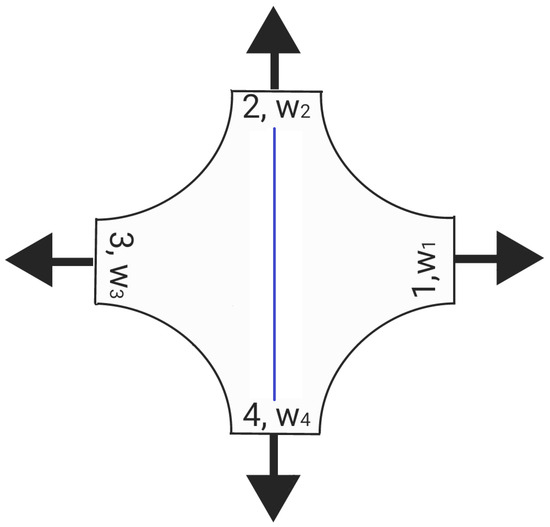
\includegraphics[width=0.3\linewidth]{img/malt_dirichlet.png}};
\node[boxL, below=8mm of fe, minimum width=46mm] (data) {Сбор данных\\ $D(p,w)=\{(C,S)\}$};

% MIDDLE COLUMN
\node[boxM, right=28mm of fe, minimum width=54mm] (xi) {деформация Лапласа\\ $\boldsymbol{\xi}=\boldsymbol{\xi}(C)$};
\node[boxM, below=8mm of xi, minimum width=54mm] (arch) {Архитектура CLaNN\\ $\psi_{\rm phys}(\boldsymbol{\xi})$};
\node[boxM, below=8mm of arch, minimum width=54mm] (smap) {Автодифференцирование \\ $S=\partial\psi/\partial C$};
\node[trainbox, below=8mm of smap, minimum width=54mm] (train) {Обучение\\ $L=\|\vect S_{pred}-\vect S\|_{L2}$ (Adam)};

% RIGHT COLUMN
\node[boxR, right=28mm of arch, minimum width=50mm] (gh) {Производные\\ $g(\xi),\ H(\xi)$};
\node[boxR, below=8mm of gh, minimum width=50mm, minimum height=36mm] (infl) {FE-раздутие\\ рексация + Ньютон\\[2pt]
  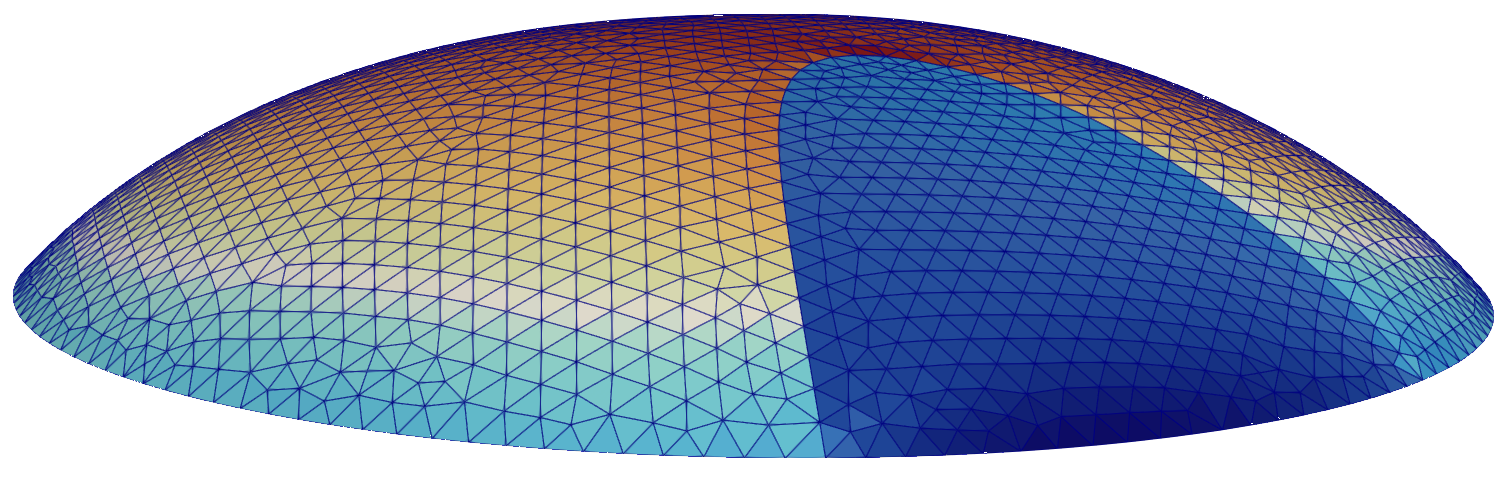
\includegraphics[width=0.3\linewidth]{img/Numerical/het/plane.png}};

% ORTHOGONAL ARROWS
\draw[->] (fe) -- (data);
% вилка от датасета: одна ветвь к деформации, другая — к обучению
\path (data.east) -- ++(10mm,0) coordinate (datasplit);
\draw[->] (data.east) -- (datasplit) |- (xi.west);
\draw[->] (datasplit) |- (train.west);
\draw[->] (xi) -- (arch);
\draw[->] (arch) -- (smap);
\draw[->] (smap) -- (train);
\draw[->] (arch.east) -- (gh.west);
\draw[->] (gh.south) -- (infl.north);
% пунктир: обновление параметров из обучения обратно в архитектуру (слева)
\draw[dashedarrow] (train.west) -- ++(-8mm,0) |- (arch.west);

\end{tikzpicture}
}
  \caption{Схема вычислительного контура CLaNN.}
  \label{fig:clann_pipeline}
\end{figure}

Такое построение архитектуры CLaNN обеспечивает выполнение всех необходимых физических свойств гиперупругой модели: 
\textbf{термодинамическая корректность} достигается через строгое соблюдение соотношения \eqref{eq:chain-rule}, 
что гарантирует консервативность напряжений $\oint \vect{S}:\mathrm{d}\vect{C} = 0$ и согласованность с законами 
термодинамики; 
\textbf{материальная устойчивость} обеспечивается и существенно улучшается за счёт строгой выпуклости функции энергии 
$\psi(\boldsymbol{\xi})$, гарантируемой архитектурой ICNN ($\vect{W}_2 \ge 0$, выпуклая неубывающая активация); 
\textbf{объективность} автоматически выполняется благодаря параметризации через тензор 
Коши-Грина $\vect{C} = \vect{F}^{\top}\vect{F}$, обеспечивая инвариантность относительно поворотов и симметрию напряжений; 
\textbf{строгая неотрицательность и коэрцитивность энергии} обеспечиваются архитектурной калибровкой 
$\psi_{\mathrm{phys}}(\boldsymbol{\xi}) = \mathbf{W}_2^{\top}(z - z_0) - \mathbf{r}_0^{\top}\boldsymbol{\xi}$,
что даёт $\psi_{\mathrm{phys}}(\mathbf{0})=0$, $\psi_{\mathrm{phys}}(\boldsymbol{\xi})>0$ при $\boldsymbol{\xi}\ne\mathbf{0}$ и 
$\psi_{\mathrm{phys}}(\boldsymbol{\xi})\to\infty$ при $\|\boldsymbol{\xi}\|\to\infty$; 
% \textbf{численная стабильность} достигается через логарифмическую параметризацию Лапласа \eqref{eq:laplace_coords}, которая корректно обрабатывает большие деформации и предотвращает нефизичные значения; 
наконец, \textbf{физические ограничения} \eqref{eq:energy_constraints} обеспечиваются архитектурой сети CLaNN: монотонные, выпуклые функции активации,
неотрицательные весовые коэффициенты, центрирование энергии деформации $\psi$ и отклика $\vect r$.



\section{Виртуальный эксперимент}

Для обучения и тестирования CLaNN мы использовали синтетические  данные двухосного растяжения и раздувания гиперупругой мембраны соответственно.
% Мы используем синтетические экспериментальные данные для тестирования CLaNN 
% на изотропном надуваним однородной и неоднородной по толщине мембраны. 
% А именно, мы генерируем данные с помощью виртуальных экспериментов на плоских растяжениях образца и используем их в качестве входных данных для 
% обучения CLaNN, без какого-либо дополнительного знания об изотропности/анизотропии образца и форме потенциала.
Обучение модели проводилось на численных экспериментальных данных, 
полученных при двухосном растяжении образца с геометрией "мальтийский крест" и толщиной $H=0.53$ мм (Рисунок \ref{fig:malt_geometry}) методом гиперупругой узловой силы \cite{ddaniso2024}. 
Материал мембраны задавался неогуковской моделью \cite{ogden1997nonlinear} \eqref{eq:neo_hookean_energy}:
\begin{align} \label{eq:neohook}
        \widetilde{\psi} &= \dfrac{\mu H(X)}{2} (I_1 +J^{-2}-3),
        \quad     I_1 = e^{2\xi_1} (1+\xi_3^2)+e^{2\xi_2},\quad J = e^{\xi_1+\xi_2}
\end{align}
с $\mu=0.43\cdot 10^6$ Па.

% Данные для обучения извлекались из различных областей образца...

% Для решения задачи равновесия гиперупругой мембраны используется метод описанный в \cite{ddaniso2024}.

\begin{figure}[H]
  \centering
  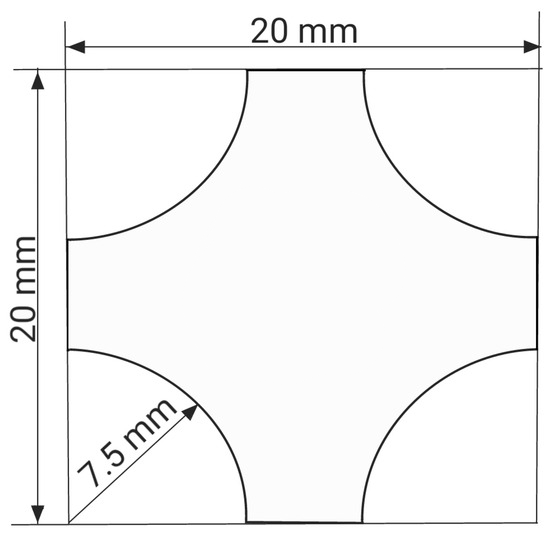
\includegraphics[width=0.4\textwidth]{img/malt_geom.png}
  \caption{Размеры образца биоматериала в форме мальтийского креста. 
  Радиус вырезов одинаков для всех вырезов}
  \label{fig:malt_geometry}
  \label{fig:malt_displacements}
\end{figure}

Схема нагружения образца показана на рисунке \ref{fig:malt_displacements}, где $w_i \in [0,1]$, $i \in \{1,4\}$
представляет собой долю от заданного максимального смещения $u_{\max}$ для $i$-го плеча: $w_i = 0$ 
соответствует неподвижному плечу, а $w_i = 1$ — соответствует плечу, чьё положение было сдвинуто и фиксировано на расстояние $u_{max}$. 
Изменяя $w_i$, можно получить различные варианты двухосного нагружения. 
В наших виртуальных экспериментах мы последовательно
смещаем плечи с приращением $\Delta s$. 
Смещение $w_i \cdot n \cdot \Delta s$ прикладывается к $i$-му плечу на $n$-м шаге, где $n = 1, \ldots, N$, 
$N = u_{\max}/\Delta s$ — количество шагов. 
Метод гиперупругой узловой силы применялся к изначально плоской квазиоднородной неструктурированной триангуляции с шагом сетки $h=0.5$ мм и размером $5 404$ треугольников. Максимальное смещение плеча
$u_{\max} = 2$ мм и $\Delta s = 0.2$ мм.
На каждом шаге извлекались $\mathbb{C}, \mathbb{S}$ для всех треугольников, принадлежащих выбранной области наблюдения. 
% Поскольку мы используем линейные ($P_1$) конечные элементы, значения $(\vect C, \vect S)$ постоянны на каждом треугольнике.

 
 
Наш предлагаемый тестовый протокол предполагает девять экспериментов:

\begin{table}[H]
\centering
\caption{Протоколы тестовых экспериментов}
\label{tab:test_protocols}
\begin{tabular}{|c|c|c|c|c|}
\hline
\textbf{№} & $w_1$ & $w_2$ & $w_3$ & $w_4$ \\
\hline
1 & 1 & 1 & 1 & 1 \\
2 & 1 & 0.75 & 1 & 0.75 \\
3 & 0.75 & 1 & 0.75 & 1 \\
4 & 1 & 0.5 & 1 & 0.5 \\
5 & 0.5 & 1 & 0.5 & 1 \\
6 & 1 & 1/3 & 1 & 1/3 \\
7 & 1/3 & 1 & 1/3 & 1 \\
8 & 1 & 0 & 1& 0 \\
9 & 0 & 1 & 0 & 1 \\
\hline
\end{tabular}
\end{table}

\subsubsection{Правила отбора данных}
\paragraph{Центральное окно $w$.}
Окно задаётся в исходной конфигурации $\Omega_0$ как центральная область вокруг геометрического центра образца, согласованная с осями расчётной сетки.
Для $w=\text{1-элемент}$ берётся единственный центральный треугольник (ячейка, чей барицентр ближайший к центру $\Omega_0$).
Для $w=5\times5$ мм и $w=10\times10$ мм берётся квадрат со сторонами 5 и 10 мм соответственно, центрированный в центре образца; для $w=\text{всё поле}$ — вся область $\Omega_0$.
Наблюдения включают все треугольники, барицентры которых $\mathbf{X}_T$ лежат внутри выбранного окна $\mathcal{W}_w\subset\Omega_0$.
% TODO: добавить мощность окна в элементах сетки

\paragraph{Состав наблюдений (данные).}
На каждом шаге нагружения $n=1,\dots,N$ и для каждого треугольника $T\in\mathcal{T}_w$ (ячейки, попавшие в окно) фиксируется пара $(\vect C_T^{(n)},\,\vect S_T^{(n)})$, 
где $\vect C$ — правый тензор Коши–Грина, $\vect S$ — второй тензор Пиолы–Кирхгофа.
Единицы: размеры окна — мм; $\vect C$ — безразмерен; $\vect S$ — МПа. 
При этом количество элементов сетки в окне наблюдения $|\mathcal{T}_w|$ для различных окон различно: 
$1$ для $w=\text{1-элемент}$, $252$ для $w=5\times5$ мм, $954$ для $w=10\times10$ мм и $5404$ для $w=\text{всё поле}$.

\paragraph{Формирование выборок.}
Для фиксированных $(p,w)$ совокупность всех пар $(\vect C_T^{(n)},\,\vect S_T^{(n)})$ образует базовый набор $D(p,w)$, из которого формируются разбиения $D_{\mathrm{tr}}(p,w)$ и $D_{\mathrm{val}}(p,w)$.
Для заданных протокола $p$ (см. табл.~\ref{tab:test_protocols}) 
и окна центральной области образца 
$w\in\{\text{1-элемент},\,5\times5\,\text{мм},\,10\times10\,\text{мм},\,\text{всё поле}\}$ обозначим
\[
  D_{\mathrm{tr}}\equiv D_{\mathrm{tr}}(p,w),\qquad D_{\mathrm{val}}\equiv D_{\mathrm{val}}(p,w),
\]
где $D_{\mathrm{tr}}$ — обучающая, $D_{\mathrm{val}}$ — валидационная выборки.

Например, |D(\{1..10\}, \text{1-элемент})|= 90 точек данных правого тензора деформаций Коши-Грина $\vect C$ 
и второго тензора напряжений Пиолы-Кирхгофа $\vect S$ (Рисунок \ref{fig:training_data}).

\begin{figure}[H]
  \centering
  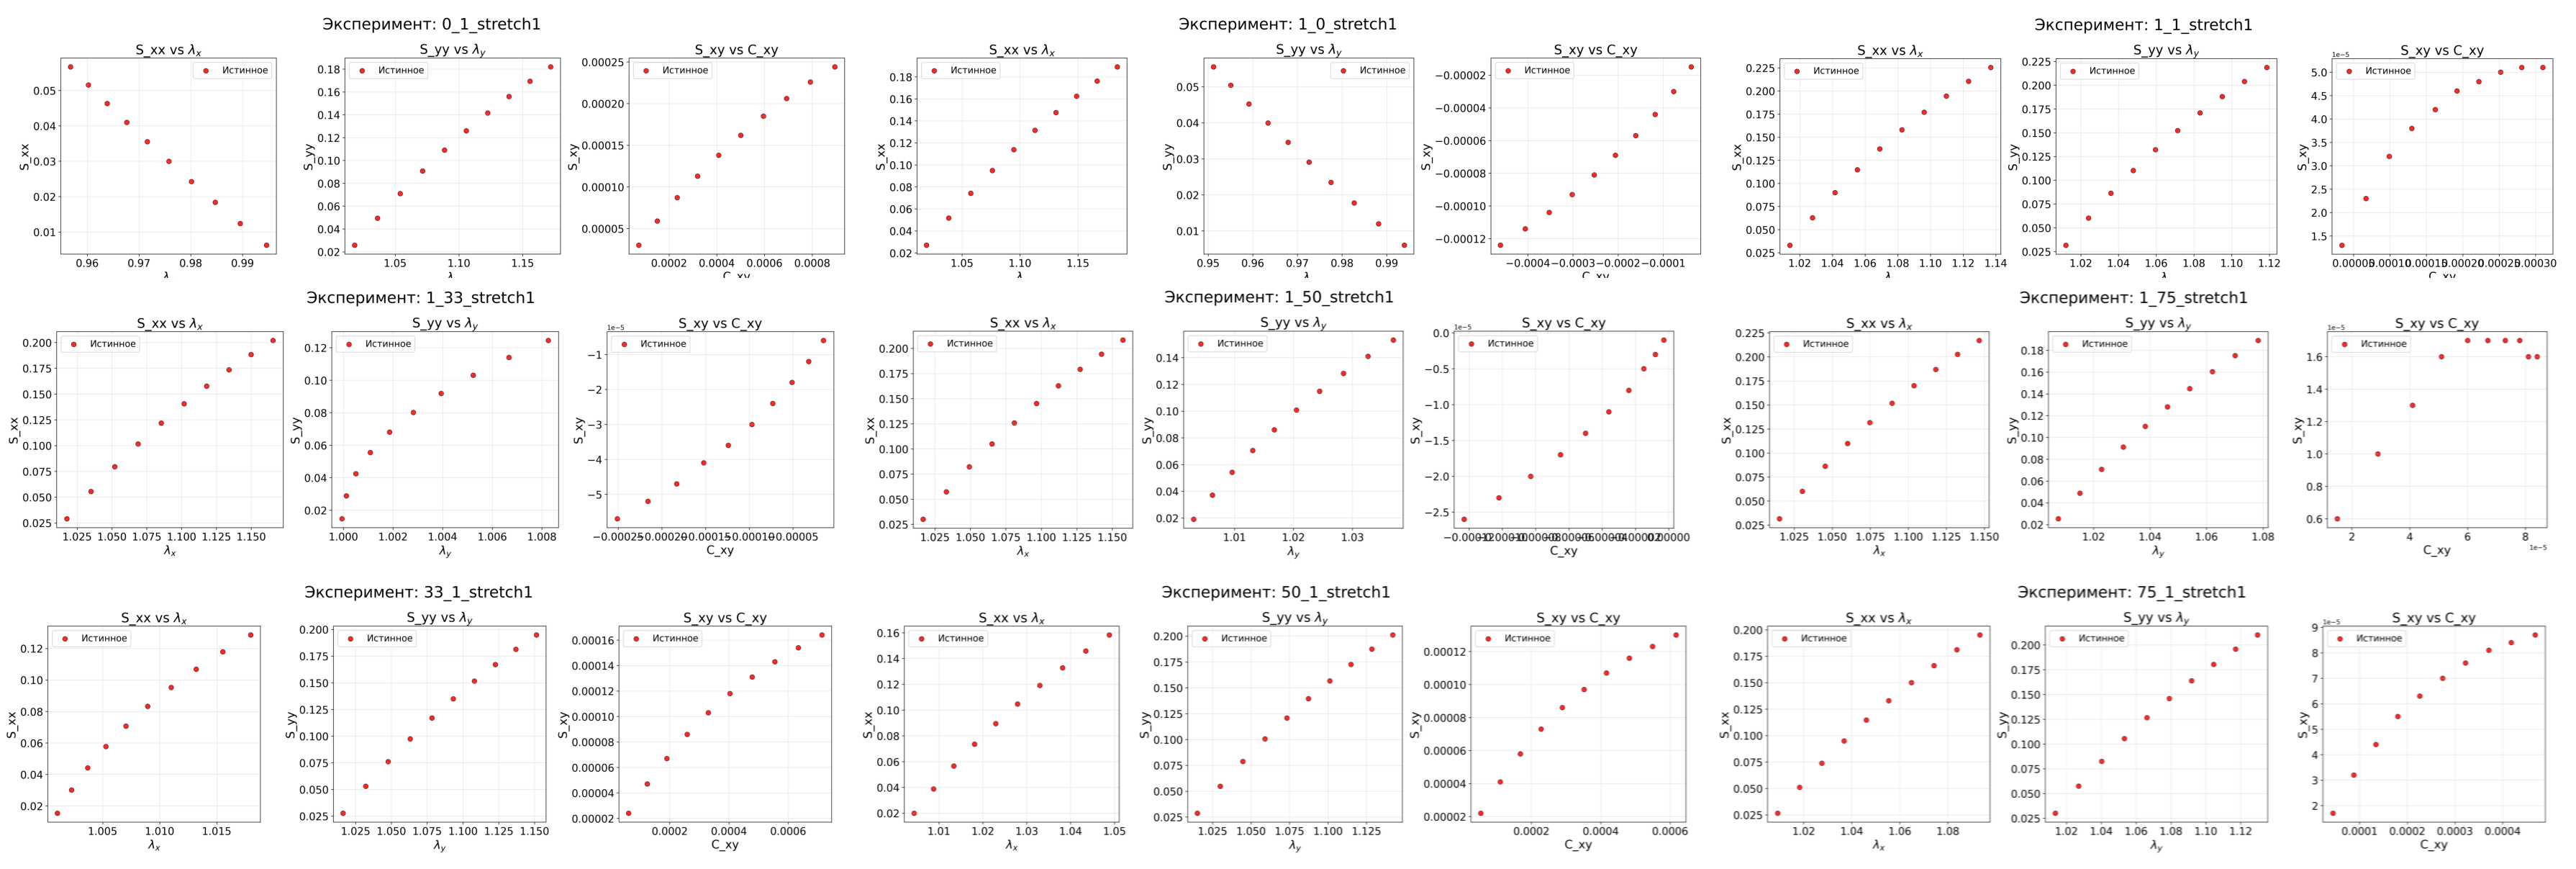
\includegraphics[width=1.0\textwidth]{img/all_stress_plots.png}
  \caption{Обучающий набор данных}
  \label{fig:training_data}
\end{figure}

Так как мы собираем данные из одного центрального элемента сетки, то растягивающие компоненты $xx, yy$ тензоров деформации $\vect C$ и напряжения
$\vect S$ имеют значения на 2-3 порядка большие чем сдвиговые компоненты $xy$.

\subsubsection{Метрики и критерии качества}
\label{sec:metrics}

Для количественной оценки качества предсказаний используем интегральные и точечные метрики, согласующиеся с энергетической нормой из вариационной постановки задач упругости (см., например, \cite{ciarlet1988mathematical,ogden1997nonlinear,holzapfel2000nonlinear}).

\textbf{Коэффициент детерминации $R^2$.}
\begin{equation}\label{eq:r_squared}
  R^2 = 1 - \frac{\sum_{i=1}^n (y_i - \hat{y}_i)^2}{\sum_{i=1}^n (y_i - \bar{y})^2},
\end{equation}
где $y_i$ — экспериментальные значения, $\hat{y}_i$ — предсказания модели, $\bar{y}$ — среднее экспериментальных значений, $n$ — число точек. Назначение: удобно сравнивать кривые нагружения; даёт нормированную меру согласия по траекториям.

\textbf{Точечная относительная ошибка.}
\begin{equation}\label{eq:rel_error}
  \epsilon = \frac{\| \vect S - \vect S_{\text{ref}} \|}{\| \vect S_{\text{ref}} \|}.
\end{equation}
% Назначение: отрисовка поля ошибки и его локальной структуры; наглядна на картах.

\textbf{P1-ошибка} \cite{xie2024p1} — комбинация абсолютной и относительной ошибок, чувствительная к малым значениям:
\begin{equation}\label{eq:p1_error}
  \epsilon_{\mathrm{P1}} = \frac{\| \vect S - \vect S_{\text{ref}} \|}{s_0 + \| \vect S_{\text{ref}} \|},\qquad s_0 = \max(\vect S_{\text{pred}}).
\end{equation}

\textbf{Абсолютная интегральная ошибка (L2 по сетке) для напряжений (Фробениус-норма).}
\begin{equation}\label{eq:l2_abs_stress}
  \|e\|_{L^2} = \Bigg( \sum_{K} \overline{\| \vect S_{\text{ref}} - \vect S_{\text{pred}} \|_F^{2}}^{\,K}\, |K| \Bigg)^{\tfrac12},
\end{equation}
где $|K|$ — мера ячейки (объём/площадь/длина). Для ячеечных данных усреднение по ячейке не требуется:
\begin{equation}\label{eq:l2_abs_stress_cell}
  \|e\|_{L^2} = \Bigg( \sum_{K} \| \vect S_{\text{ref},K} - \vect S_{\text{pred},K} \|_F^{2}\, |K| \Bigg)^{\tfrac12}.
\end{equation}
Назначение: сворачивает поле ошибки в скаляр и инвариантна к измельчению сетки (при фиксированном поле) \cite{BrennerScott2008,AinsworthOden2000,Verfurth2013}.

\textbf{Относительная интегральная ошибка.}
\begin{equation}\label{eq:l2_rel_stress}
  \|e\|_{L^2,\,\mathrm{rel}}\;=\; \frac{\Big( \sum\limits_{K} 
  \| \vect S_{\mathrm{ref},K} - \vect S_{\mathrm{pred},K} \|_F^{2}\, |K| \Big)^{\tfrac12}}
  {\Big( \sum\limits_{K} \| \vect S_{\mathrm{ref},K} \|_F^{2}\, |K| \Big)^{\tfrac12}}\,.
\end{equation}
% Назначение: корректное сопоставление сценариев с разными уровнями напряжений; нормировка на «энергетическую мощность» эталонного поля.


\textbf{Гиперпараметры оптимизации:}
\begin{itemize}
  \item Скорость обучения (learning rate): $0.001$
  \item Размер батча (batch size): $4$ при обучении на 90 точек данных и $128$ для остальных обучающих наборов данных.
  % \item Веса физических ограничений: $\lambda_{\text{SI}} = 0.1$, $\lambda_{\psi} = 0.1$
  \item Архитектура: 16 нейронов на скрытом слое
  \item Сглаживающий параметр $\beta$: $10$
\end{itemize}

\textbf{Результаты обучения:}
Процесс оптимизации показал высокую эффективность: ошибка аппроксимации снизилась на 5 порядков за менее чем 5000 эпох (рисунок \ref{fig:loss_curve}), 
что демонстрирует как качество предложенной архитектуры, так и корректность выбора гиперпараметров. 
Столь быстрая сходимость обусловлена строгой выпуклостью функции энергии, что обеспечивает единственность 
минимума и отсутствие локальных минимумов в пространстве параметров.

\begin{figure}[H]
  \centering
  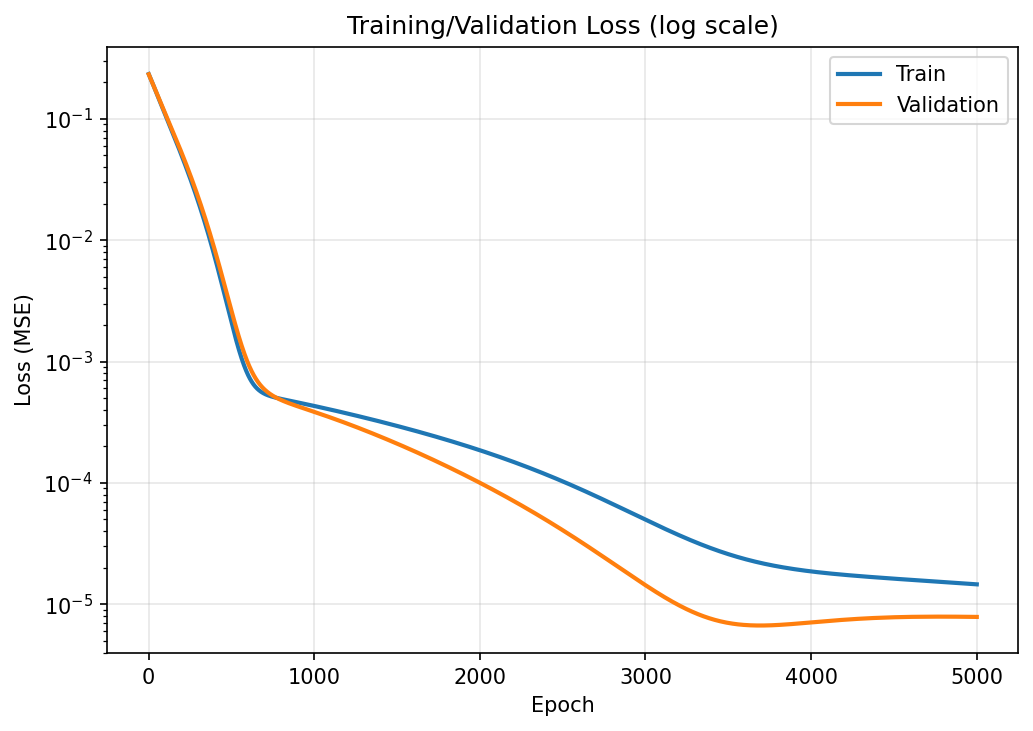
\includegraphics[width=0.7\textwidth]{img/loss_curve.png}
  \caption{Кривая функции потерь при обучении на 90 точках данных}
  \label{fig:loss_curve}
\end{figure}


\subsection{Интерполяция и экстраполяция кривых нагружения}
  Сначала мы проверили, как модель CLaNN интерполирует и экстраполирует кривые нагружения, используя выборки
  $D_{\mathrm{tr}}(p,w)$ и $D_{\mathrm{val}}(p,w)$ для заданного окна наблюдения $w$.
  Для оценки качества использовали коэффициент детерминации $R^2$ (см. раздел \ref{sec:metrics}, формулу \eqref{eq:r_squared}). Метрику качества фиксируем как:
\[
  R^2_{\alpha}(D_{\mathrm{val}}),\qquad \alpha\in\{xx,yy,xy\}.
\]

  \textbf{Интерполяция.}  

  Для тестирования спосбности архитектуры CLaNN к интерполяции кривых нагружения мы использовали данные из 
  10 точек кривой нагружения равнодвухосного растяжения мембраны $p=1$, 
  окно наблюдения $w=\text{1-элемент}$:
  
  $D_{in} = D(p{=}1,\,w{=}\text{1-элемент}),\, n = 1..10,$
  
  $D_{\mathrm{tr}}=\{\forall (\vect {C}^{n_{tr}}, \vect{S}^{n_{tr}}) \in D_{in}|\; n_{tr}=\{1,5,10\}\},$
  
  $D_{\mathrm{val}}=\{\forall (\vect {C}^{n_{val}}, \vect{S}^{n_{val}}) \in D_{in}|\; n_{val}=n \backslash  n_{tr}\}.$

  CLaNN показал высокую точность интерполяции кривой нагружения равнодвухосного растяжения мембраны 
  для растягивающих компонент $R^2_{xx}=0.999$, $R^2_{yy}=0.999$, и отсуствие достоверного предсказания сдвиговых 
  компонент $R^2_{xy}=0$ (рисунок \ref{fig:interpolation}).
  
  \begin{figure}[H]
    \centering
    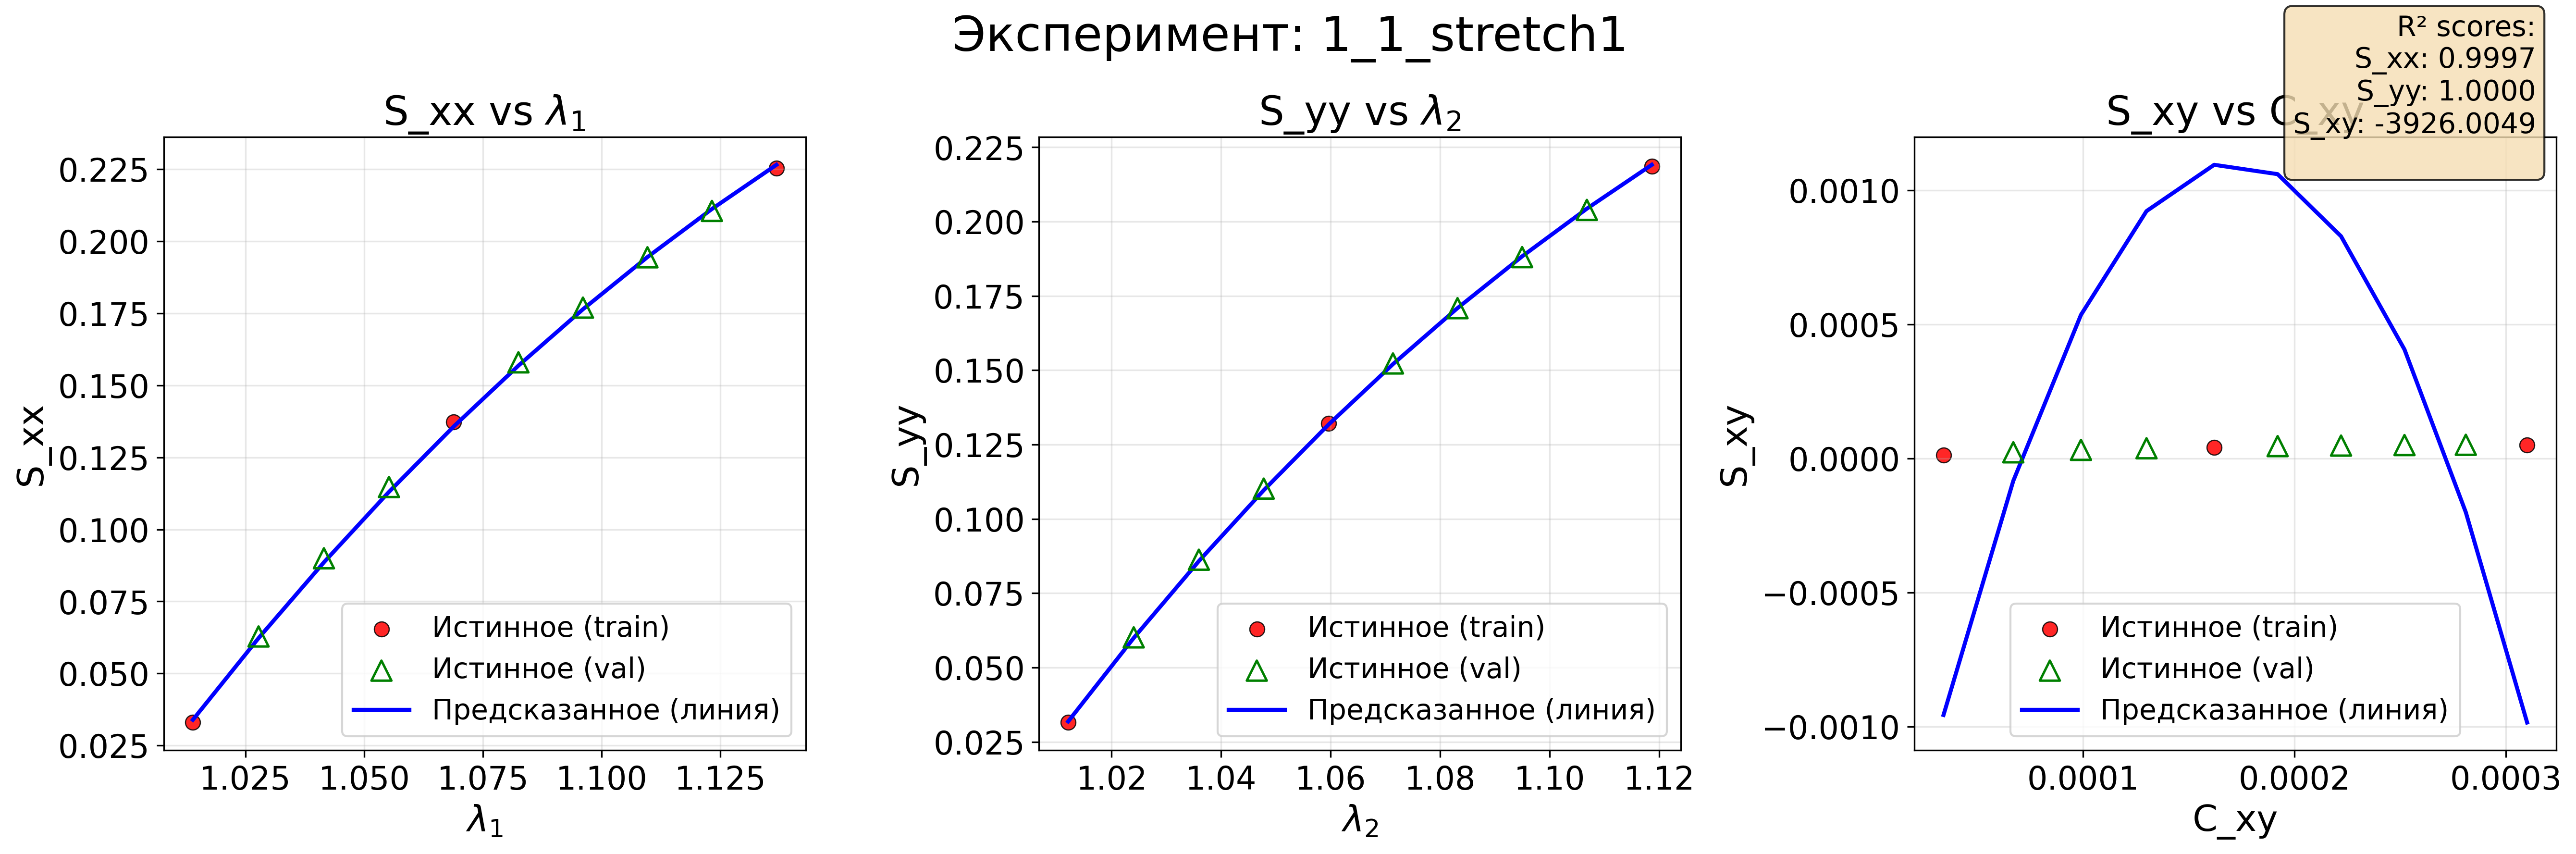
\includegraphics[width=1.0\textwidth]{img/interpolation.png}
    \caption{Кривая нагружения для равнодвухосного растяжения}
    \label{fig:interpolation}
  \end{figure}
  
  \textbf{Экстраполяция.}
  
  Для проверки способности CLaNN к экстраполяции кривых нагружения использовали обучение на равнодвухосном растяжении (p = 1) и валидацию на неравнодвухосном (p = 9), 
  окно наблюдения $w=\text{1-элемент}$:
  
  $D_{\mathrm{tr}} = D(p{=}1,\,w{=}\text{1-элемент}),\, n = 1..10,$
  
  $D_{\mathrm{val}} = D(p{=}9,\,w{=}\text{1-элемент}),\, n = 1..10,$
  
  CLaNN показал высокую точность экстраполяции для растягивающих компонент $R^2_{xx}=0.993$, $R^2_{yy}=1.0$, и отсутствие достоверного предсказания сдвиговой компоненты $R^2_{xy}=0$ (рисунок \ref{fig:extrapolation}).


  \begin{figure}[H]
    \centering
    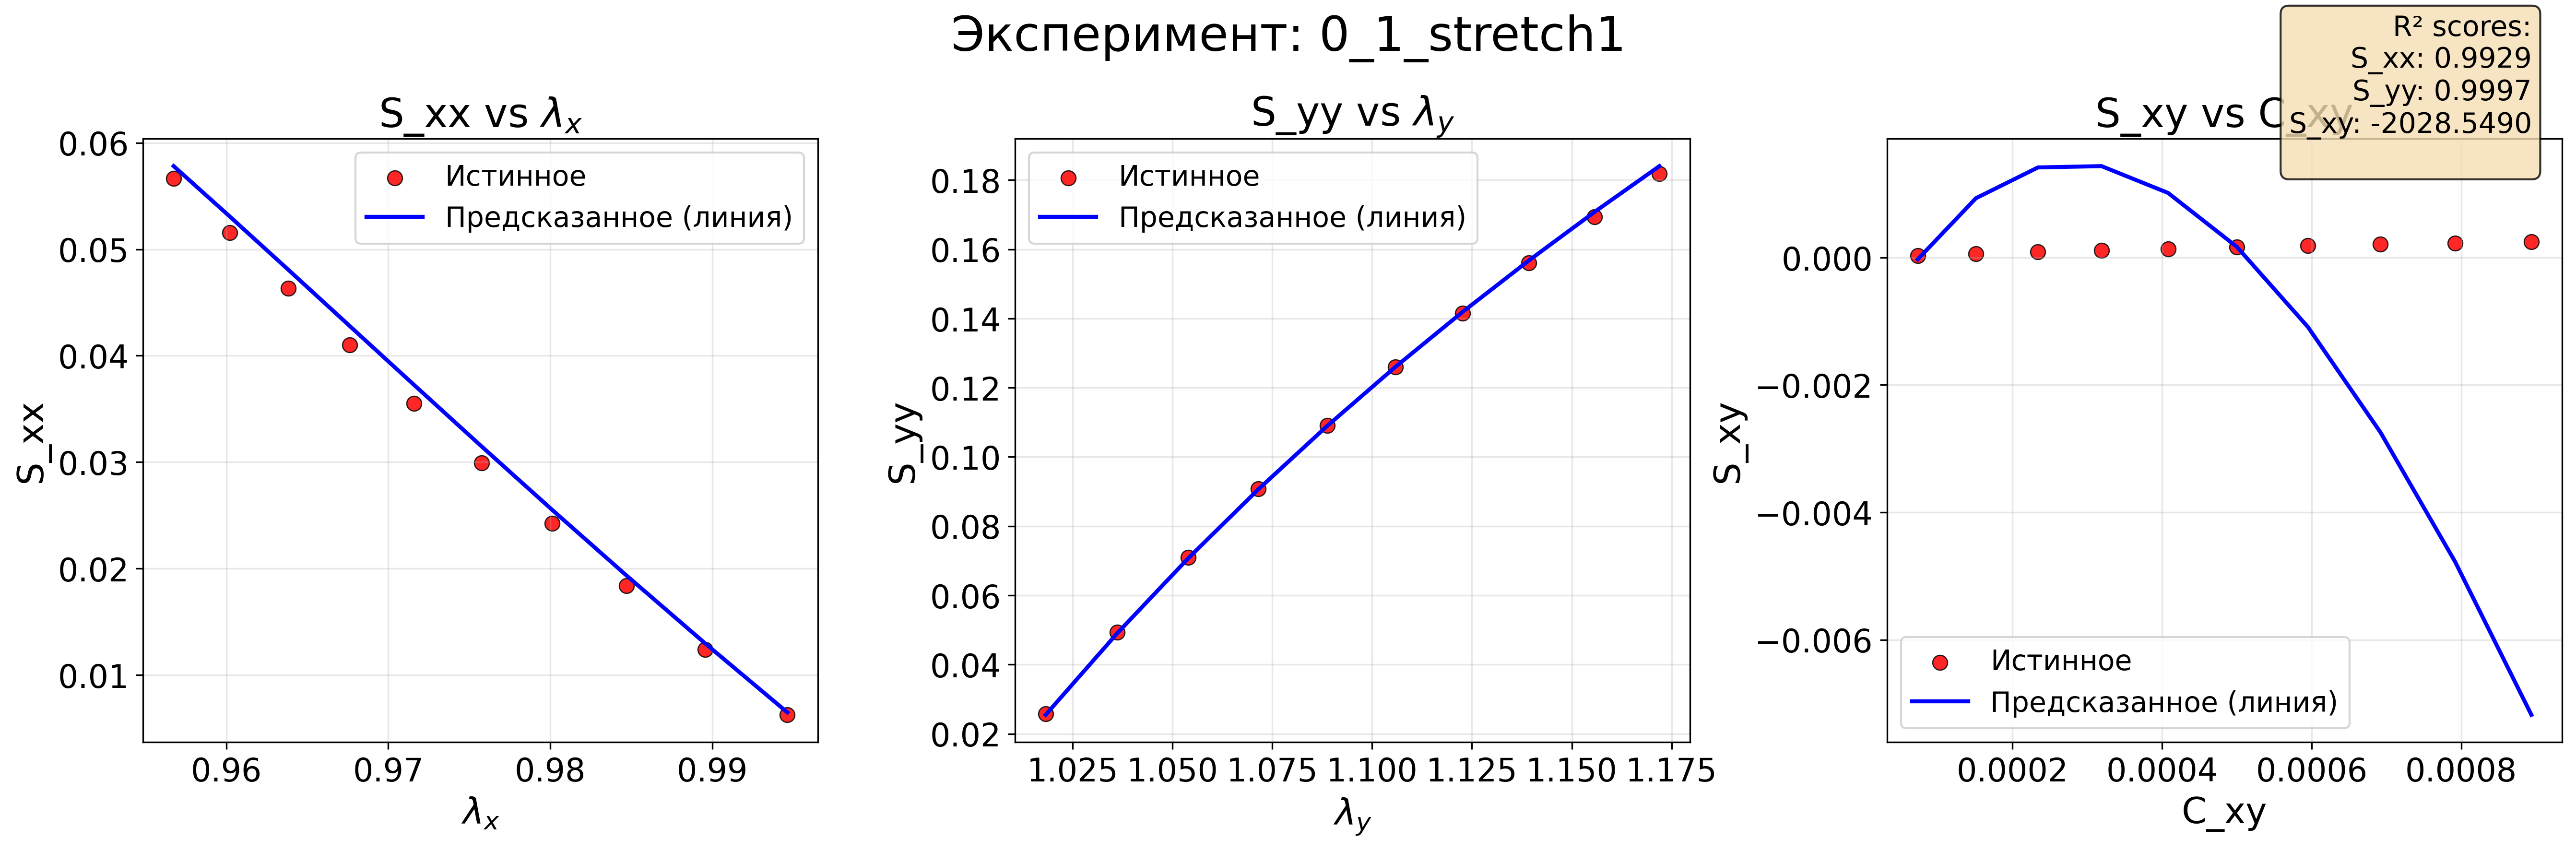
\includegraphics[width=1.0\textwidth]{img/extrapolation.png}
    \caption{Кривая нагружения для неравнодвухосного растяжения}
    \label{fig:extrapolation}
  \end{figure}
   
  Таким образом, CLaNN способен интерполировать и экстраполировать кривые нагружения с высокой точностью, что свидетельствует о его способности к обобщению на новые данные.
  Однако, не справляется с предсказанием сдвиговых компонент $\vect S_{xy}$, что может быть связано с тем, что данные для сдвиговых компонент не достаточно большие.
  
\subsection{Раздутие мембраны}

  Для проверки способности CLaNN, мы поставили численный эксперимент по раздутию круглой мембраны радиусом 25 мм.
  Мембрана закреплена по внешнему контуру и подвергается равномерному растяжению по всей поверхности при заданном давлении
  5 МПа. 
  Как референс мы использовали результаты численного эксперимента с использованием гиперупругой модели Нео-Гука с тем же параметром сдвига, 
  что и при генерации данных для обучения CLaNN.
  
  Мы использовали два поля толщин элементов $T$: 1) с гомогенным полем толищны 0.54 мм. 
  2) с гетерогенным полем толищны, где в в окружности высекается два пораболических сектора с толщиной 2 мм
  и остальной части мембраны 0.54 мм (Рисунок \ref{fig:membrane_thickness}). 

  В качестве точечной метрики используем относительную ошибку (см. раздел \ref{sec:metrics}, формулу \eqref{eq:rel_error});
  для сравнения сдвиговых компонент — P1-ошибку \cite{xie2024p1} (см. формулу \eqref{eq:p1_error}).

  \begin{figure}[H]
    \centering
    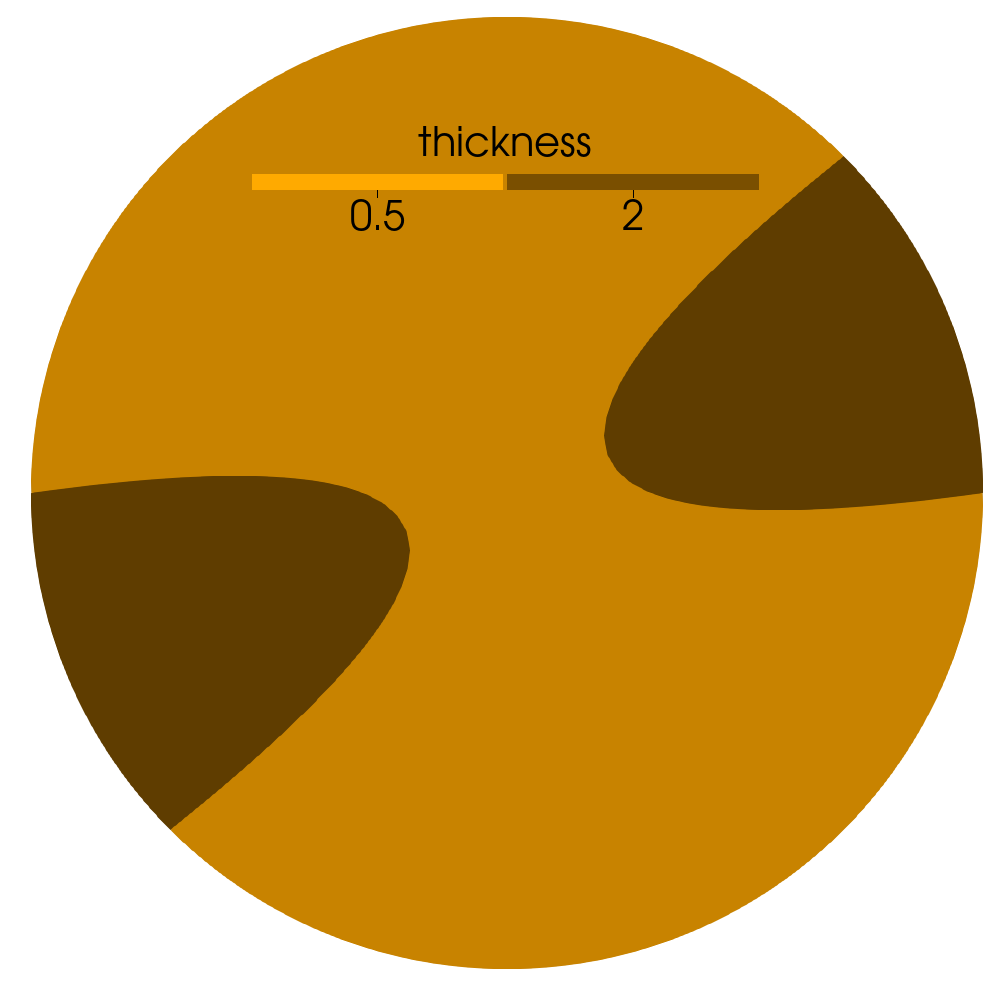
\includegraphics[width=0.25\linewidth]{img/het_circle.png}
    \caption{Гетерогенное поле толщин элементов $T$ круглой мембраны.}
    \label{fig:membrane_thickness}
  \end{figure}
  % \begin{wrapfigure}{r}{0.35\textwidth}
  %   \centering
  %   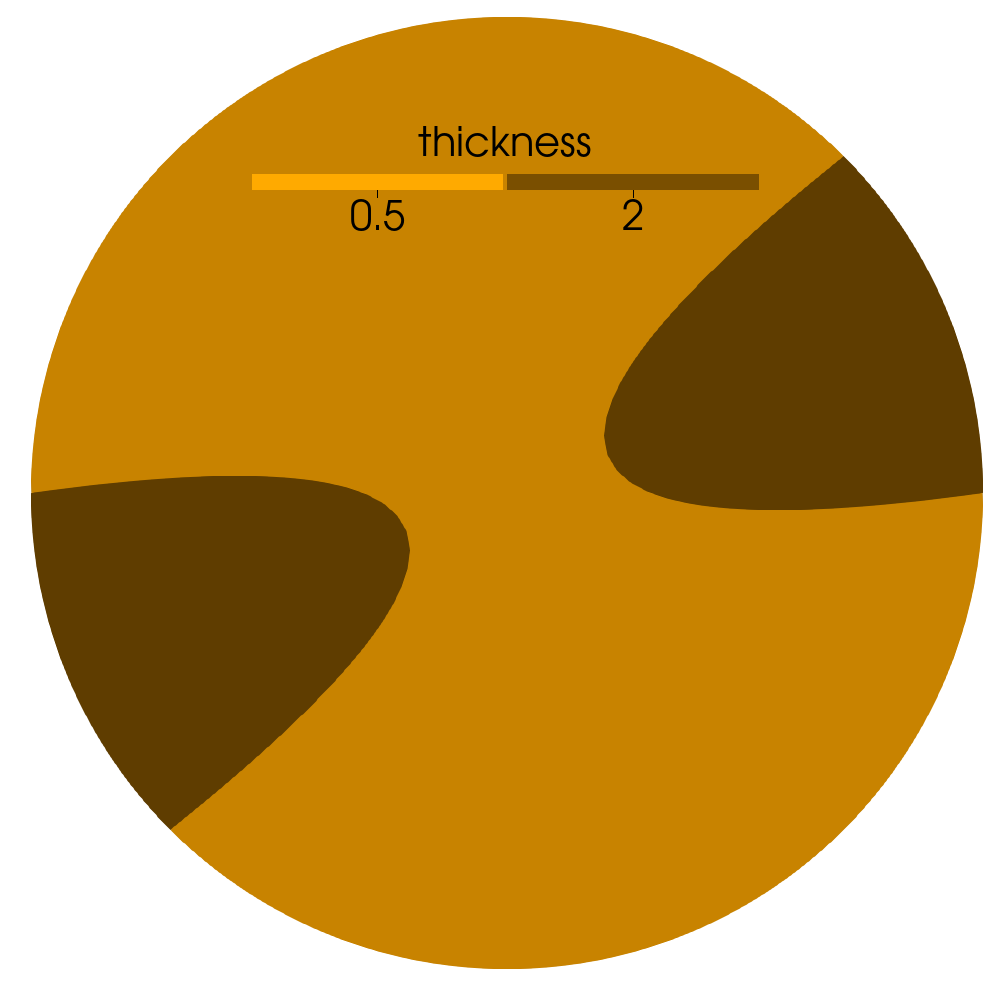
\includegraphics[width=\linewidth]{img/het_circle.png}
  %   \caption{Гетерогенное поле толщин элементов $T$ круглой мембраны.}
  %   \label{fig:membrane_thickness}
  % \end{wrapfigure}
  % Для геометрии с гетерогенным полем толщин референсные значения сдвиговой компоненты поля 2 тензора напряжений Пиолы-Кирхгофа 
  % $\vect S$ (Рисунок \ref{fig:numerical_experiment}) .

  \begin{figure}[H]
    \centering
    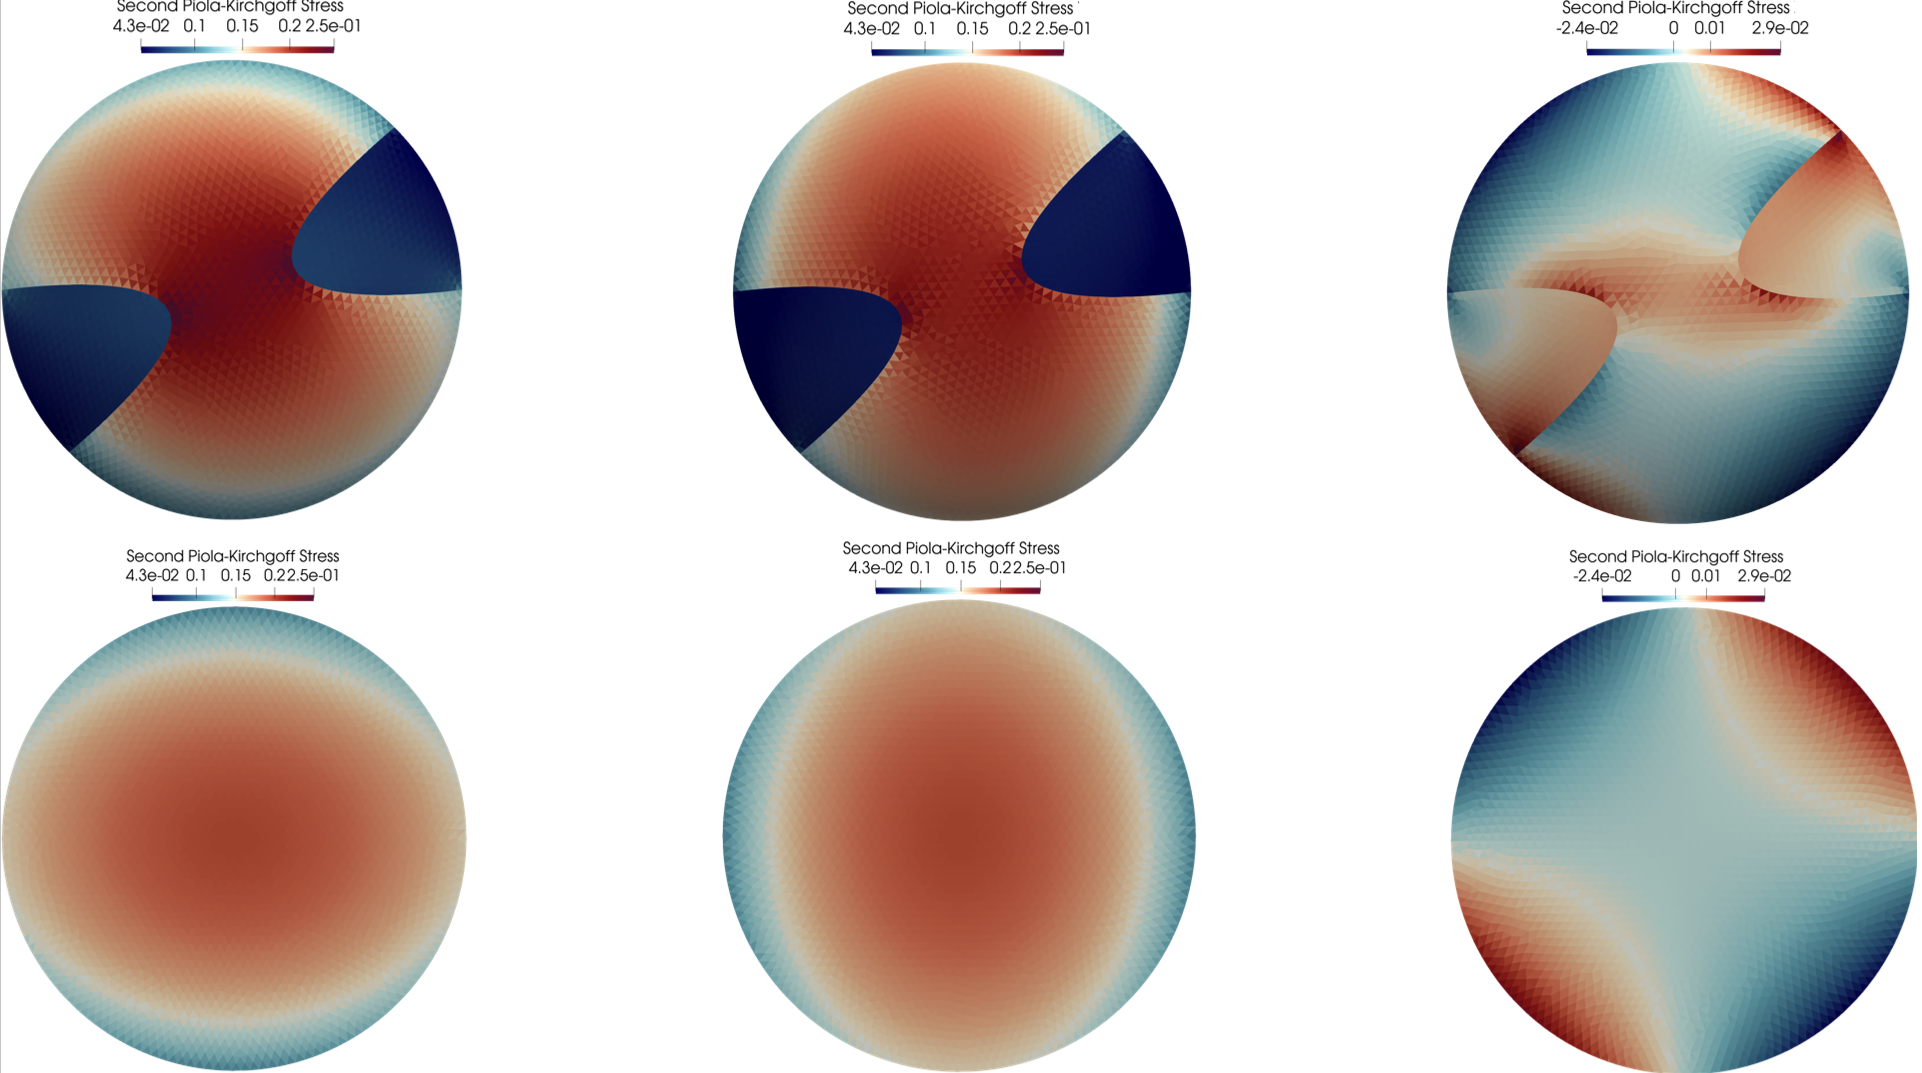
\includegraphics[width=0.7\textwidth]{img/Numerical/ref_stress.png}
    \caption{Поле напряжений $\vect S$ круглой мембраны (пример результата численного эксперимента).}
    \label{fig:numerical_experiment}
  \end{figure}
  
  В результате численного эксперимента на раздутие мембраны с гиперупругим определяющим соотношением CLaNN,
  используя набор данных $D (\{1..10\}, w=\text{1-элемент})$ для обучения, мы получили поле напряжений 2 тензора Пиолы-Кирхгофа 
  $\vect S$ для гомогенной и гетерогенной мембраны по толщине и сравнили его
  с референсными значениями (Рисунок \ref{fig:numerical_experiment}) и построили поле ошибок $\epsilon$ и $\epsilon_{P1}$ (Рисунок \ref{fig:numerical_errors}).
  Сдвиговая компонента напряжений $\vect S_{xy}$ показывает наибольшую ошибку для гетерогенной мембраны, 
  что может быть связано с тем, что данные для сдвиговых компонент не достаточно большие. Поэтому мы последовательно 
  расширяли набор данных для обучения до $D (\{1..10\}, w=\text{5x5})$, $D (\{1..10\}, w=\text{10x10})$, $D (\{1..10\}, w=\text{все поле})$, 
  и построили зависимость интегральной ошибки $\|e\|_{L^2}$ (Формула \eqref{eq:l2_abs_stress_cell}) и $\|e\|_{L^2,\,\mathrm{rel}}$ (Формула \eqref{eq:l2_rel_stress}) 
  поля напряжения $\vect S$ от размера окна наблюдения $w$ (Рисунок \ref{fig:integral_errors}). 
  В итоге абсолютная интегральная ошибка $\|e\|_{L^2}$  для гетерогенной мембраны уменьшается с увеличением размера окна наблюдения $w$, 
  это может быть связано с тем, что при увеличении размера окна наблюдения мы учитываем больше данных для обучения, в том числе данных 
  для сдвиговых компонент напряжений, например, при отборе ячеек из области ближе к углам квадрата, в который вписана мембрана, 
  сдвиговые компоненты напряжений в этой области вырастают на 1-2 порядка.
  
  
  \begin{figure}[H]
    \centering
    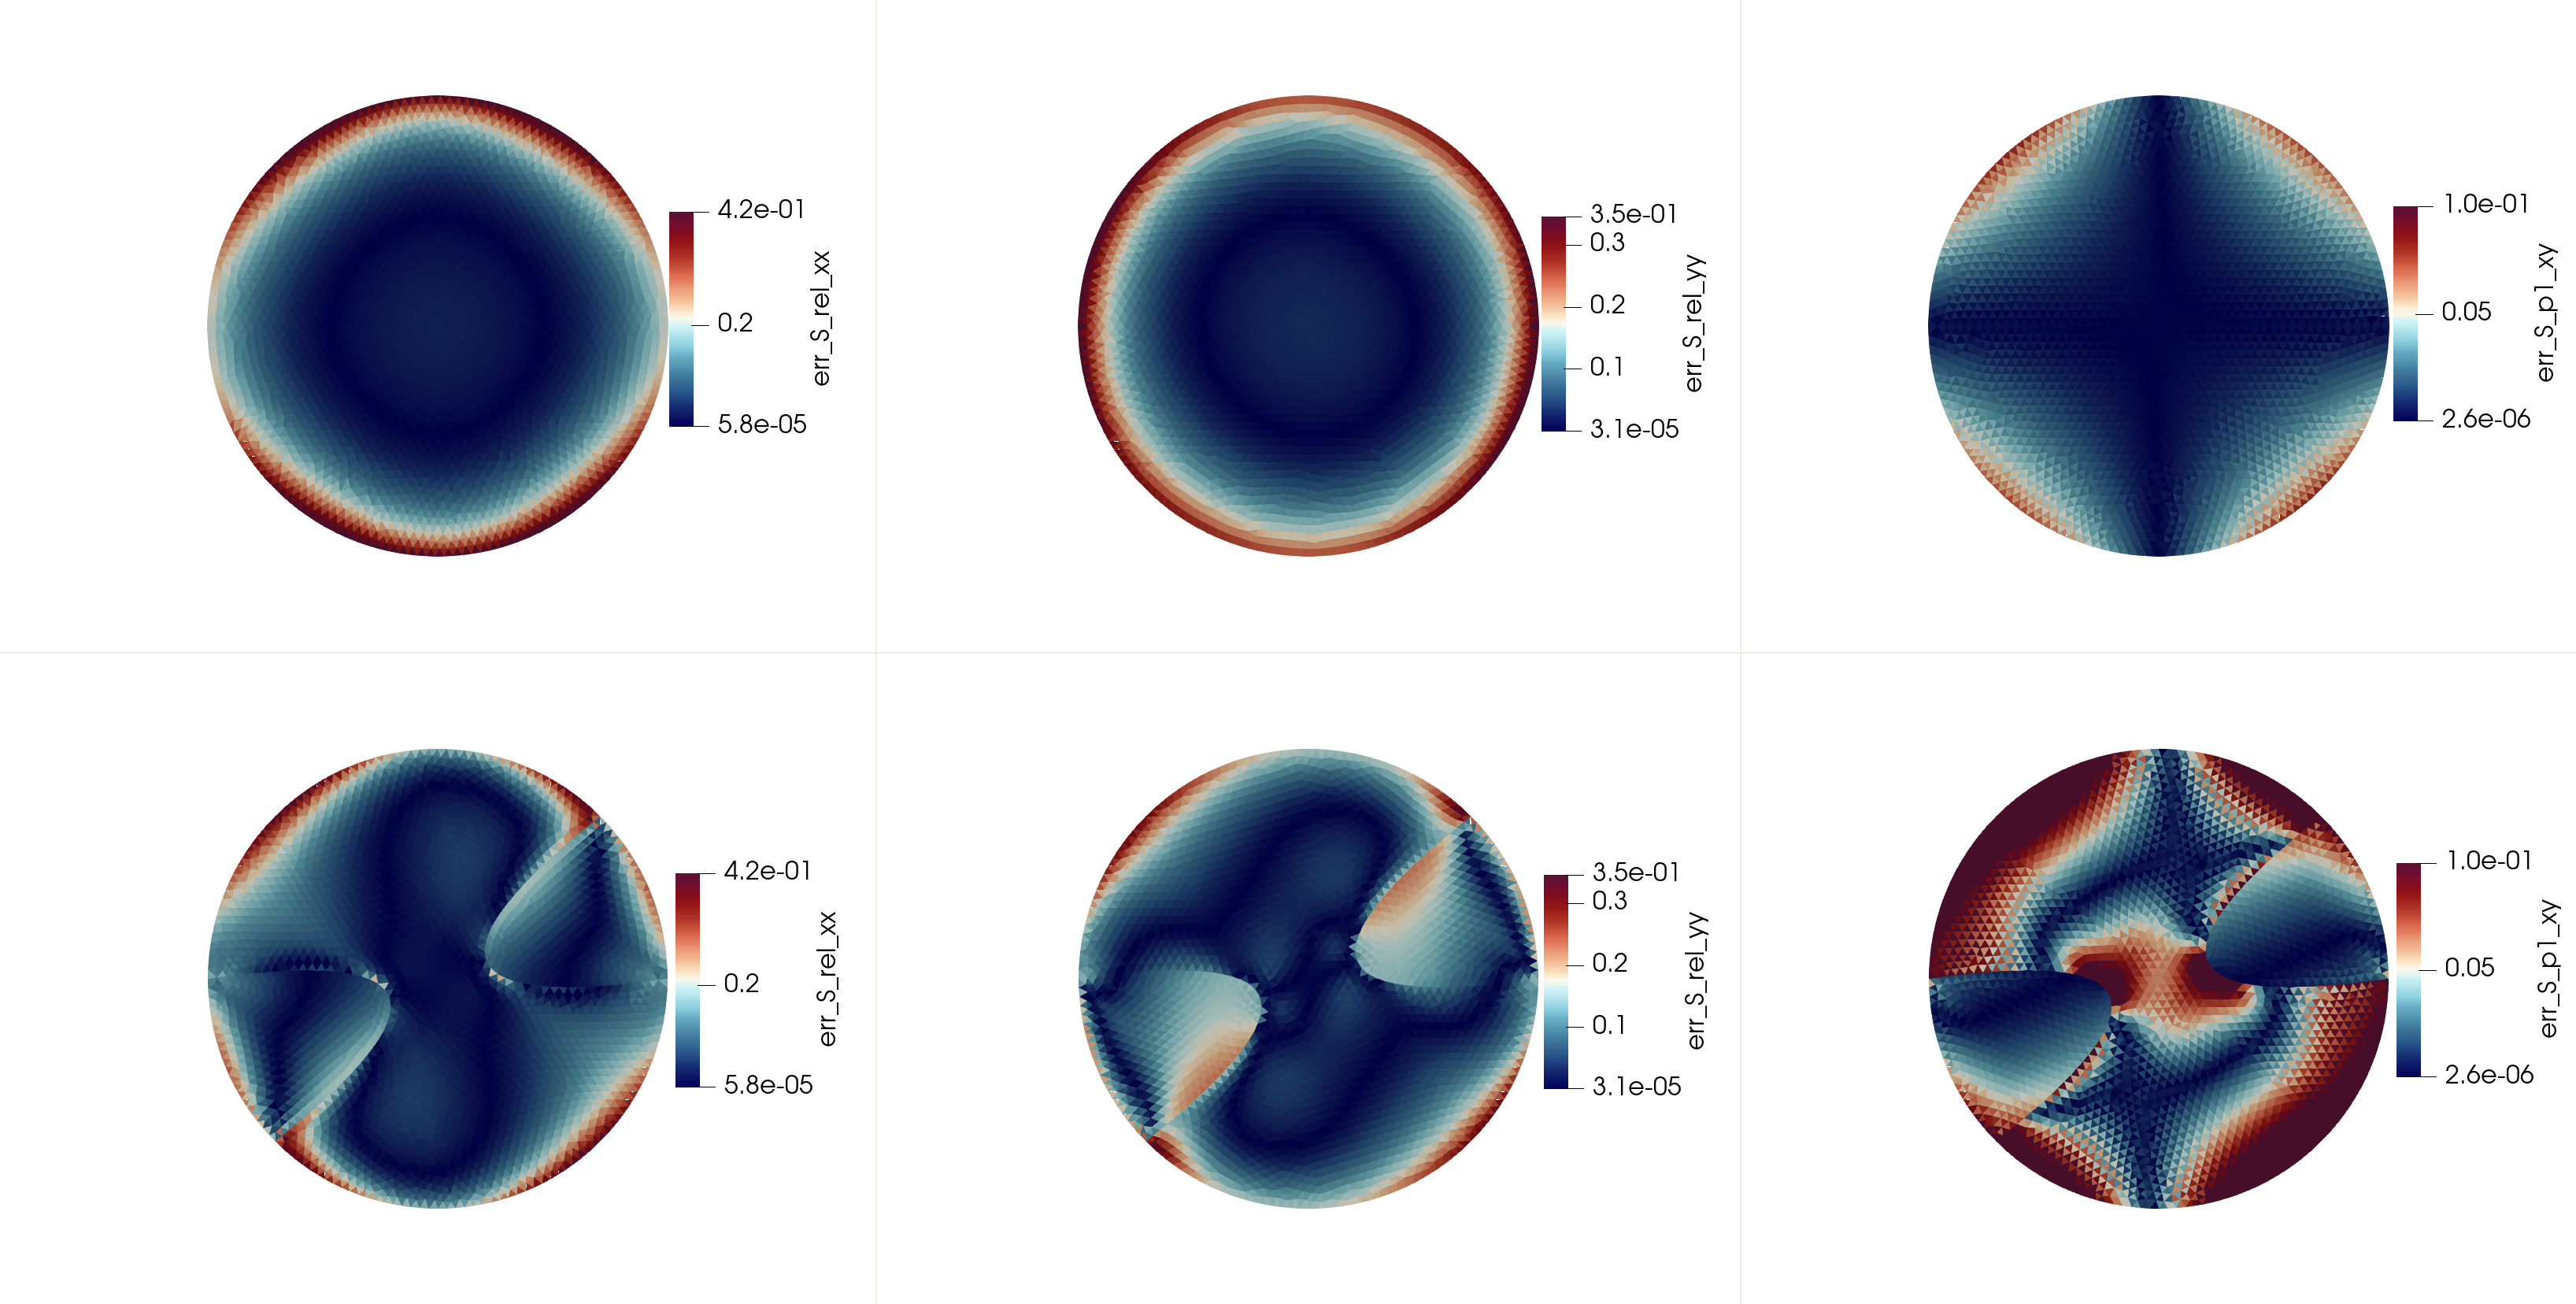
\includegraphics[width=1.0\textwidth]{img/Numerical/errs.png}
    \caption{Поле ошибок между предсказанными и эталонными значениями напряжений.}
    \label{fig:numerical_errors}
  \end{figure}

  \begin{figure}[H]
    \centering
    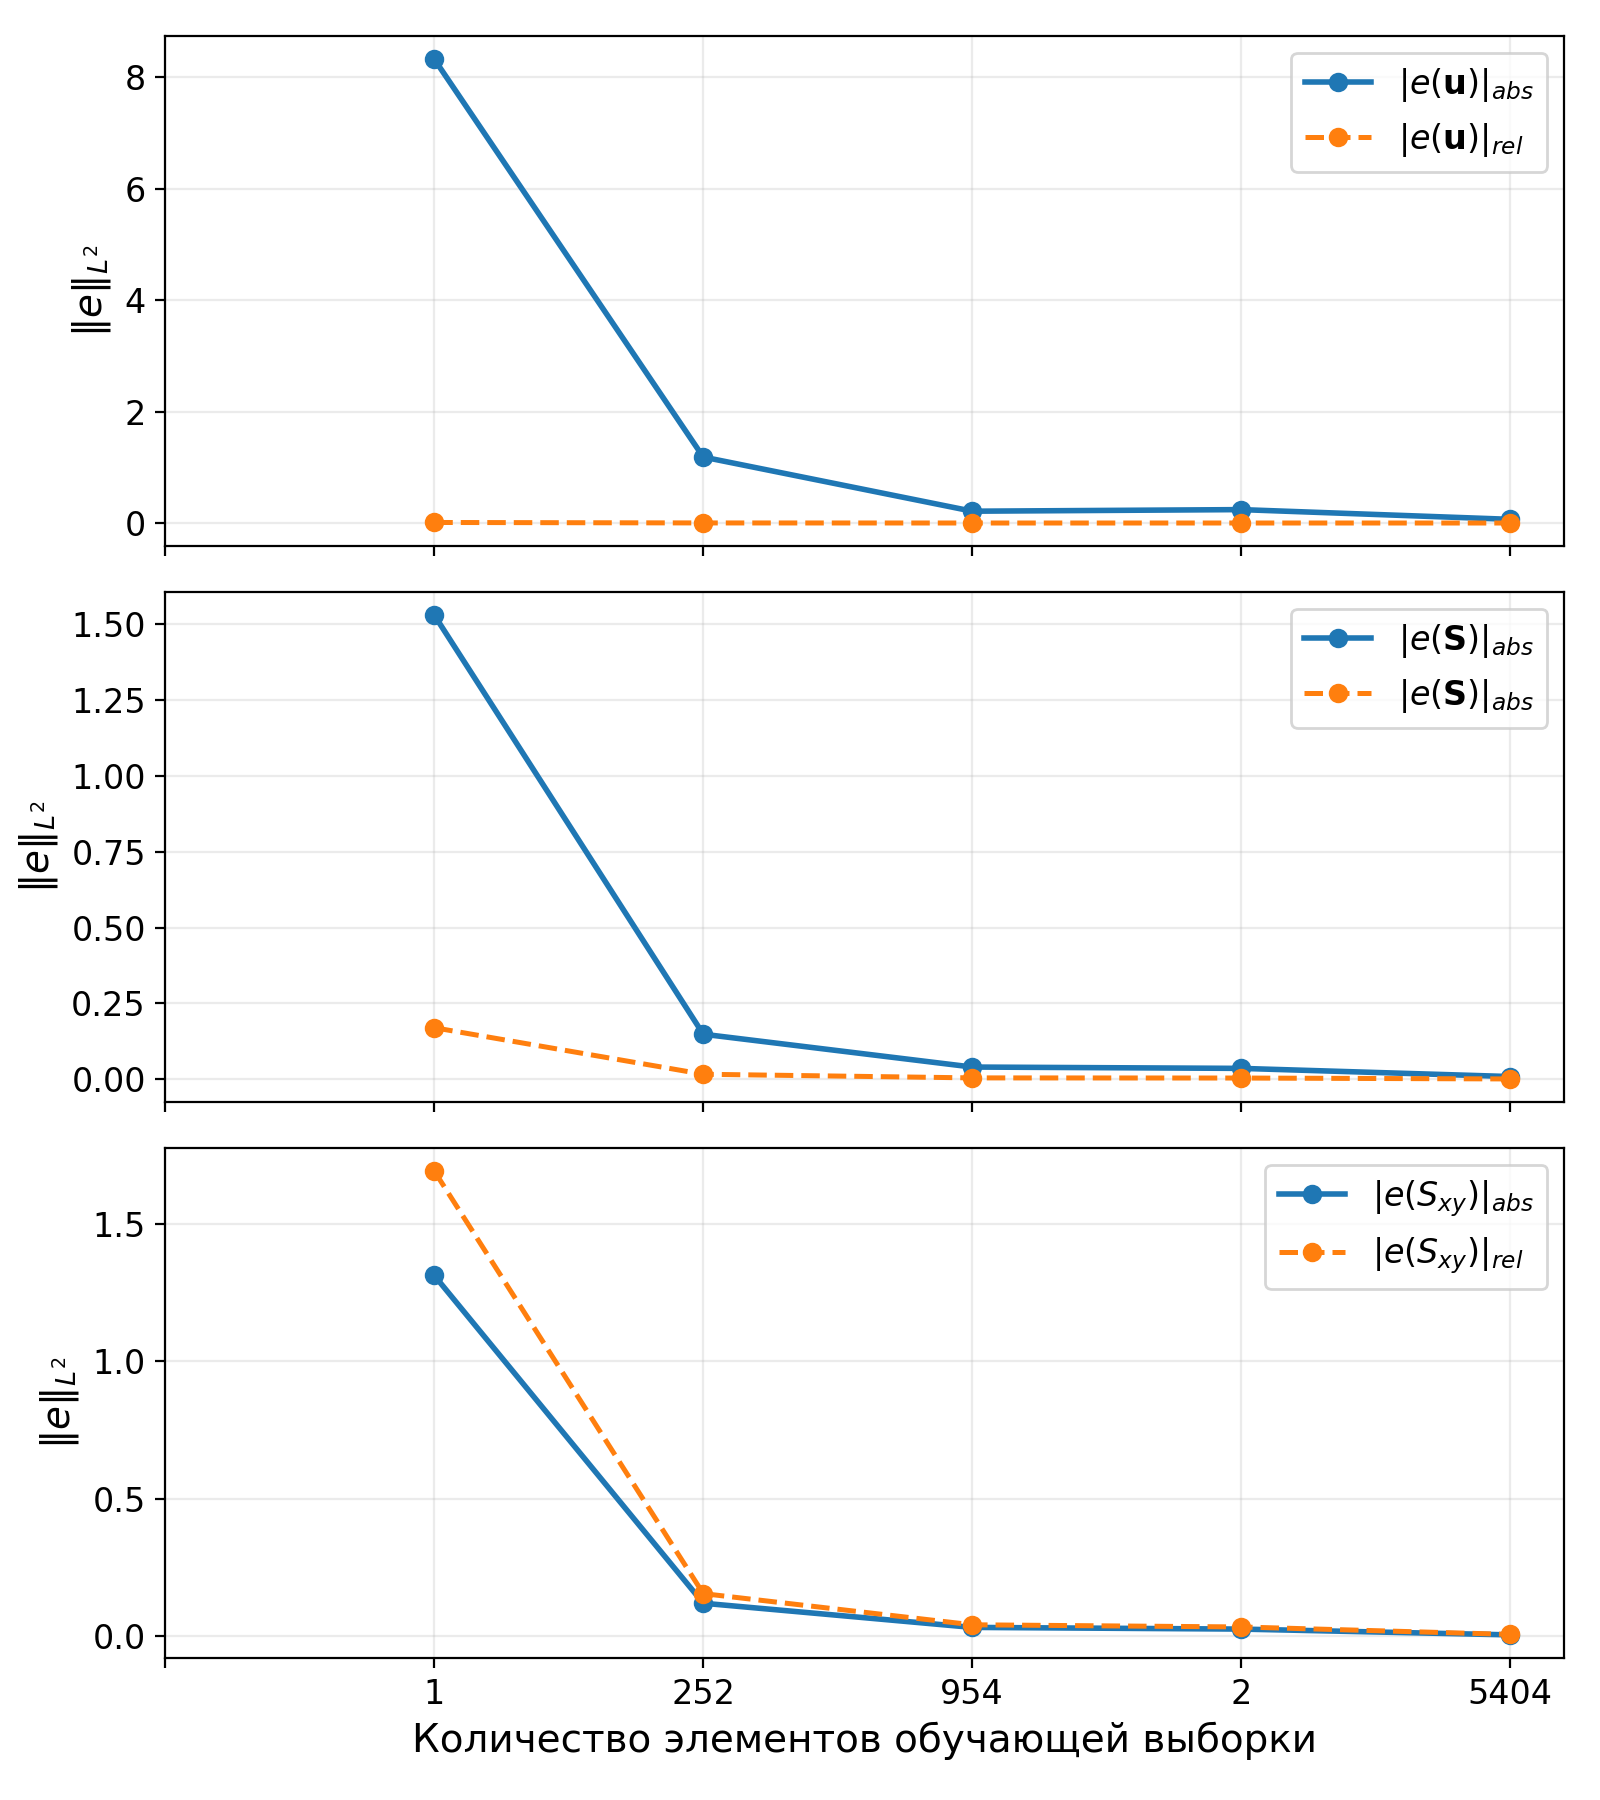
\includegraphics[width=0.5\textwidth]{img/integral_errors.png}
    \caption{Зависимость интегральной ошибки $\|e\|_{L^2}$ и $\|e\|_{L^2,\,\mathrm{rel}}$ от количества элеметов в окне наблюдения размера $w$.}
    \label{fig:integral_errors}
  \end{figure}
  
  % \begin{figure}[H]
  %   \centering
  %   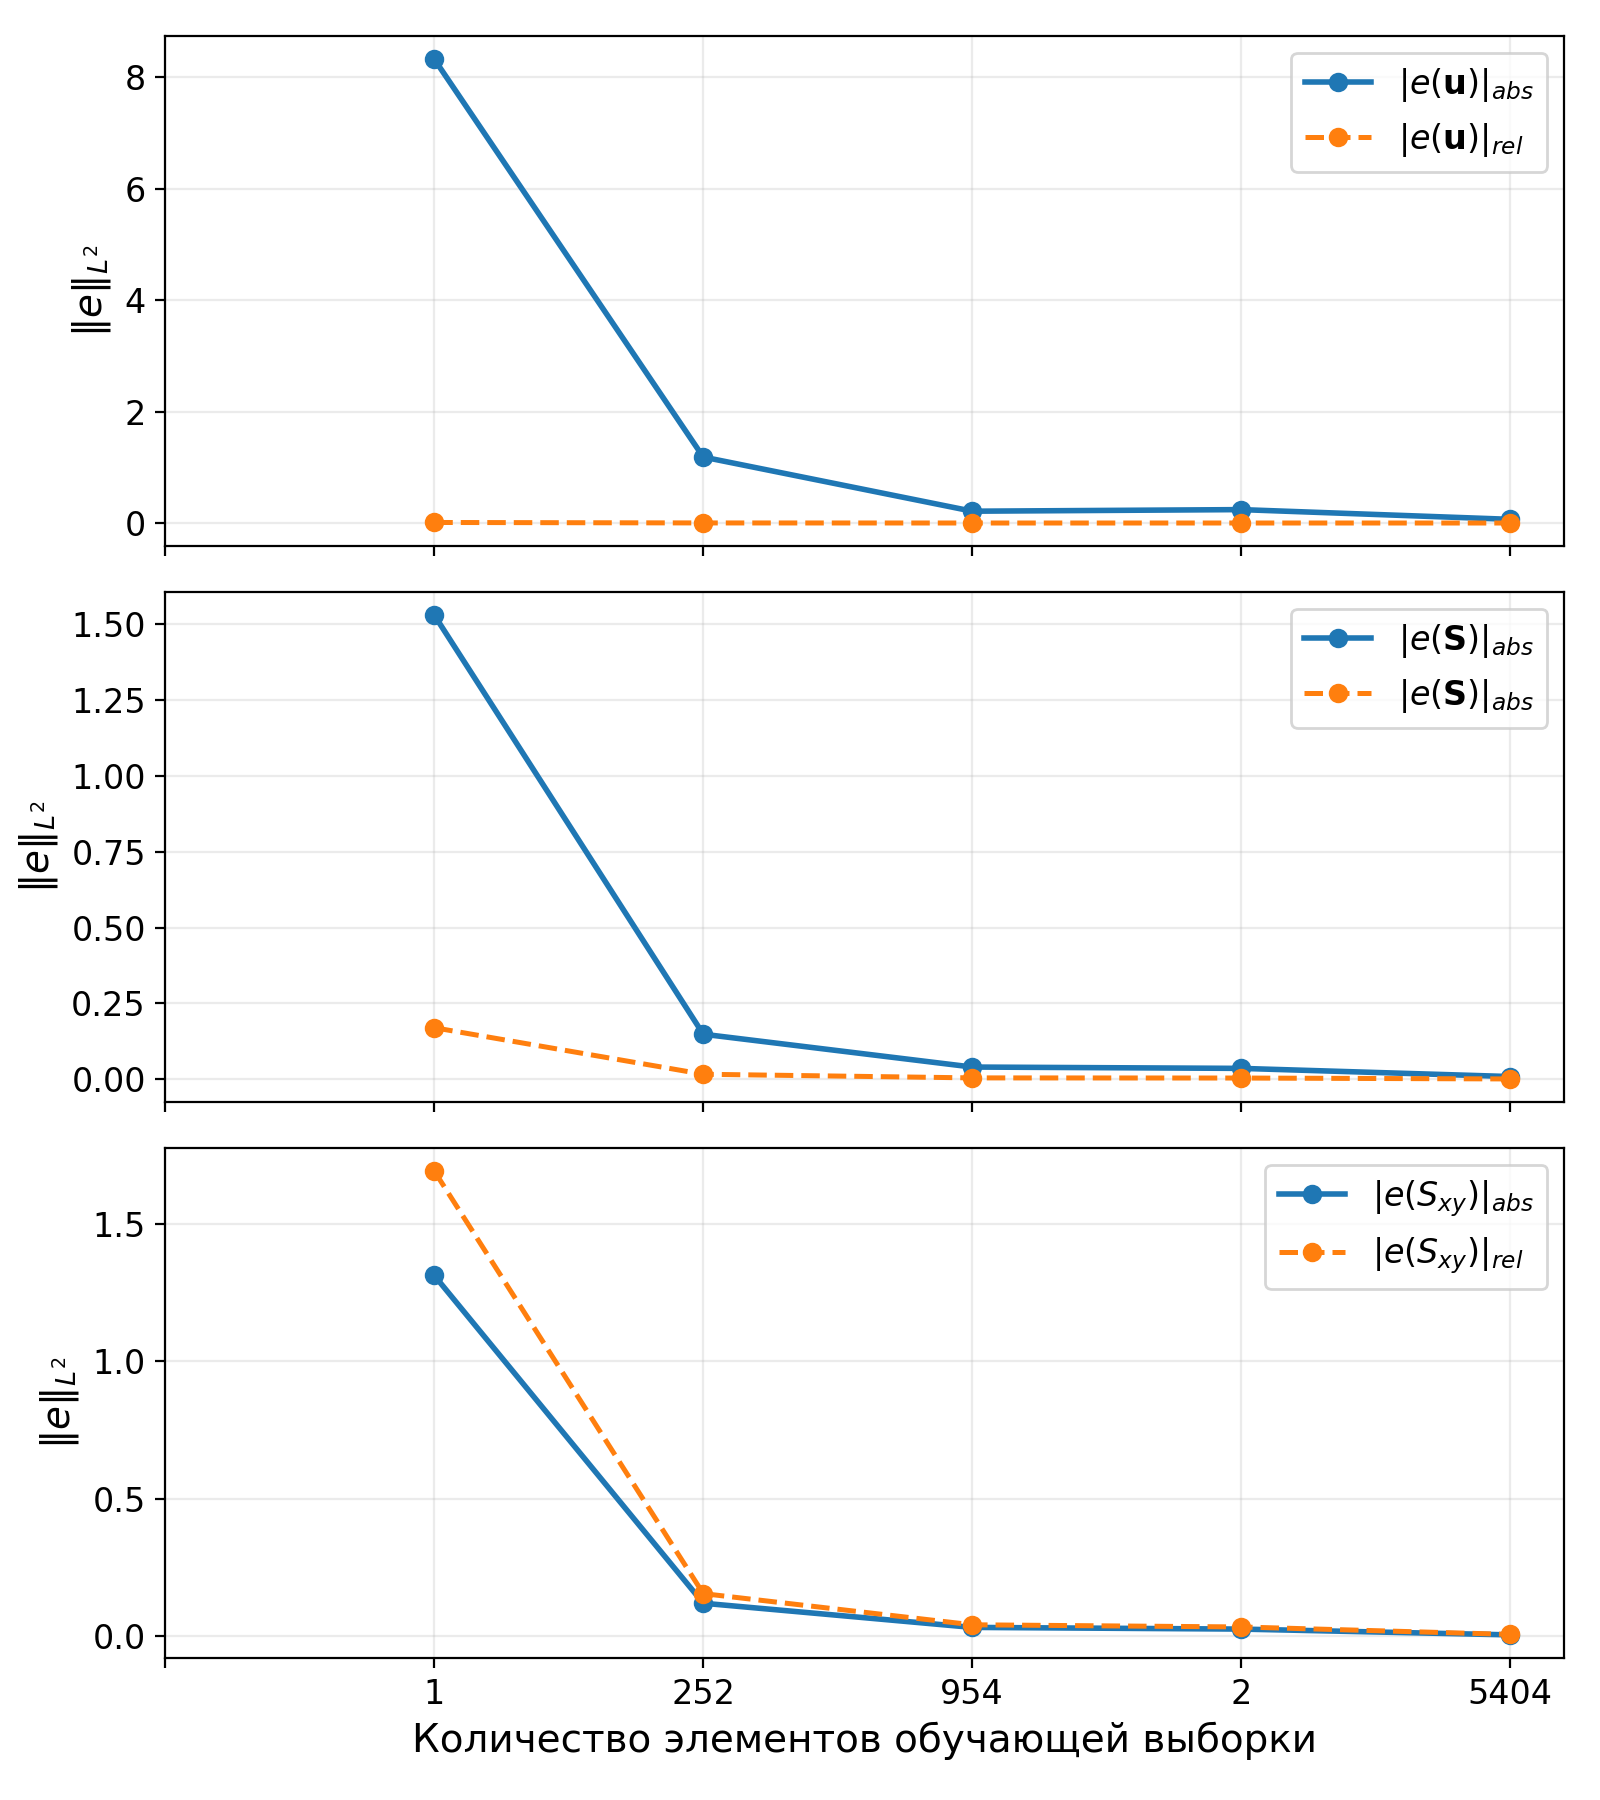
\includegraphics[width=0.7\textwidth]{img/integral_errors.png}
  %   \caption{Интегральные ошибки в зависимости от окна наблюдения.}
  %   \label{fig:_integral_numerical_errors}
  % \end{figure}
  
\subsection{Сравнение вычислительной эффективности CLaNN}

  Благодаря \emph{выпуклости} потенциальной энергии деформации $\psi(\boldsymbol\xi)$ в CLaNN задача стационарного равновесия формулируется
  как гладкая выпуклая минимизация. Это позволяет использовать градиентные и второпорядковые методы со строгими гарантиями сходимости
  (квазиньютон, Ньютона и тд)
  и предсказуемой сложностью до заданной точности \cite{BoydVandenberghe2004,Nesterov2004,NocedalWright2006,ConnGouldToint2000}.
  В окрестности минимума сильная выпуклость и липшицевость гессиана обеспечивают локально квадратичную сходимость Ньютона,
  а квазиньютоновские схемы (L\textendash BFGS) дают сверхлинейные скорости \cite{NocedalWright2006}.

  % \paragraph{Data-drevin модели без выпуклости.}
  В таблично-заданных/локально-интерполяционных DD-моделях (в т.ч.\ k-NN, IDW) выпуклость энергии, как правило, не гарантируется,
  а функция отклика может быть негладкой. Это приводит к невыпуклой постановке с множеством стационарных точек и
  отсутствием глобальных гарантий у классических квазиньютоновских методов. На практике применяются
  квазистатические/релаксационные стратегии: (добавить описание) \cite{KirchdoerferOrtiz2016,KirchdoerferOrtiz2017}.
  Такие методы устойчивы, но, как правило, требуют существенно большего числа шагов нагружения и внутренних итераций
  (а также повторяющихся k-NN/IDW-запросов), что приводит к росту времени расчёта.

  Мы сравнили время решения для CLaNN, классической гиперупругой модели Нео\textendash Гука и DD-модели мембраны, описанной в \cite{xi2023}.
  Задача: раздувание закреплённой круглой мембраны, $R{=}25$ мм, равномерное давление, две конфигурации по толщине $T$ (гомогенная и гетерогенная; см. рис.~\ref{fig:membrane_thickness}).
  Для CLaNN обучаем на наборе данных $D(\{1..10\},\,w{=}\text{1-элемент})$; для сравнения используем DD-модель на основе 
  kNN и IDW, которые работает в пространстве деформаций Лапласа и функций отклика $(\vect{\xi}, \vect{r})$, 
  которые были вычислены из $D(\{1..10\},\,w{=}\text{10}\times\text{10})$ \cite{xi2023}.
  Численное решение выполняем в одной и той же КЭ-постановке для мембранной задачи. 
  Все варианты останавливаем по одинаковым нормам допускам по невязке.

\begin{table}[htbp]
\centering
\caption{Время расчёта (сек) на задаче раздувания: гомогенная vs гетерогенная толщина}
\label{tab:experiments_summary}
\begin{tabular}{|l|c|c|}
\hline
\textbf{Метод} & \textbf{Гомогенная} & \textbf{Гетерогенная} \\
\hline
CLaNN & 512 & 329  \\
\hline
Neo-Hooke & не замерил & не замерил\\
\hline
kNN & 993 & -- \\
\hline
\end{tabular}
\end{table}

На одинаковой сетке и допусках CLaNN достигает решения сравнимым числом глобальных итераций с Нео\textendash Гуком
(за счёт выпуклости и корректной кривизны энергии в ICNN), существенно опережая DD-модель по времени расчета
за счёт отсутствия внешних проекций на данные и дорогих k-NN/IDW-запросов на каждой итерации.
Также стоит отметить невозможность расчета DD-модели на гетерогенной толщине без линейной интерполяции данных в близи нуля, 
что может происходить из-за нехватки данных для в этой области деформаций.


\section{Заключение}

  В работе предложена физически информированная архитектура CLaNN для гиперупругих материалов, основанная на выпуклой
  потенциальной энергии деформации и лог\textendash лапласовой параметризации кинематики.

  Архитектура обеспечивает термодинамическую согласованность; благодаря
  выпуклости задача решается как гладкая выпуклая минимизация с предсказуемой сходимостью градиентных и
  квазиньютоновских методов. 
  При этом в архитектуре для вычисления тензора напряжений явно не используется информация о сжимаемости/несжимаемости изотропности/анизотропности
  материала, что позволяет использовать CLaNN для решения задач с различными типами материалов.

  В тестах интерполяции CLaNN достигает малых ошибок при наличии репрезентативных обучающих данных; в режиме
  экстраполяции сохраняет устойчивость и физическую правдоподобность отклика,
  тогда как локально\textendash интерполяционные DD\textendash модели (k\textendash NN/IDW) проявляют артефакты за пределами окна обучения.

  На численных экспериментах раздувания закреплённой круглой мембраны (гомогенная и гетерогенная толщина) CLaNN корректно
  воспроизводит поля перемещений и напряжений и демонстрирует быстрое, предсказуемое сходимостное поведение в единой
  КЭ\textendash постановке для всех сравниваемых моделей.

  По вычислительной эффективности CLaNN превосходит kNN\textendash основанную DD\textendash модель: на гомогенной задаче выигрыш составляет
  порядка $\times 1.9$ за счёт отсутствия дорогостоящих k\textendash NN/IDW\textendash запросов и внешних проекций на данные на каждой итерации. 
  Стоит отметить, что полученная величина выигрыша может быть и выше за счет оптимизации взаимодействия решателя и CLaNN, а также подбора оптимальных гиперпараметров.
  На гетерогенной толщине CLaNN сохраняет работоспособность без специальных эвристик, 
  тогда как DD\textendash модель требует дополнительной регуляризации и/или интерполяции данных в окрестности малых деформаций.
  Также из-за отсутсвия критерия остановки расчета по норме невязки у релаксационных методов решения задачи равновесия может привести к сложноценимому увеличению времени расчета
  по сравнения с ньютоновскими методами, с которыми позволяет работать CLaNN.

  В итоге CLaNN объединяет механическую корректность и эффективность нейросетей: выпуклая энергия и дифференцируемость обеспечивают устойчивое 
  решение вариационных задач и ускоряют расчёт по сравнению с классическими DD\textendash подходами, а также высокую способность к аппроксимации гиперупругих материалов
  на малых выборках данных. 
  Дальнейшие направления: протестировать анизотропные материалы и реальные экспериментальные данные.


\appendix

\chapter{\texorpdfstring{Эквивалентность QR-факторизации $\vect F$ и разложения Холецкого $\vect C=\vect F^{\top}\vect F$ для вычисления логарифмических координат $\boldsymbol{\xi}$}{Эквивалентность QR и Холецкого}}
\label{app:cholesky}

\section{Постановка и обозначения}

Рассматривается двумерная гиперупругая кинематика. Пусть:
\begin{itemize}
  \item $\vect F \in \mathbb{R}^{2 \times 2}$ — градиент деформации, $\det \vect F > 0$,
  \item $\vect C = \vect F^{\top}\vect F$ — правый тензор Коши–Грина (симметричный положительно определённый, SPD),
  \item Холецкий: $\vect C = \vect U^{\top}\vect U$, где $\vect U$ — верхнетреугольная и $\text{diag}(\vect U) > 0$,
  \item Логарифмические координаты:
    $\boldsymbol{\xi} = (\xi_1, \xi_2, \xi_3) = (\ln u_{11}, \ln u_{22}, u_{12}/u_{11})$.
\end{itemize}

Цель: показать, что при наличии $\vect F$ можно заменить вычисление $\vect U = \text{chol}(\vect C)$ на $\vect U = \vect R$ из тонкого QR($\vect F$) = $\vect Q \vect R$ (с $\text{diag}(\vect R) > 0$), и получить те же $\boldsymbol{\xi}$.

\section{Теорема (эквивалентность U и R)}

Пусть $\vect F \in \mathbb{R}^{2 \times 2}$ невырождённая ($\det \vect F > 0$). Рассмотрим тонкую QR-факторизацию
\begin{equation}
\vect F = \vect Q \vect R,
\end{equation}
где $\vect Q \in \mathbb{R}^{2 \times 2}$ — ортогональная ($\vect Q^{\top}\vect Q = \vect I$), $\vect R \in \mathbb{R}^{2 \times 2}$ — верхнетреугольная. Выберем стандартную нормализацию $\text{diag}(\vect R) > 0$. Тогда $\vect R$ совпадает с фактором Холецкого для $\vect C$:
\begin{equation}
\vect R = \text{chol}(\vect C), \quad \text{с} \quad \vect C = \vect F^{\top}\vect F.
\end{equation}

\textbf{Доказательство.}
\begin{equation}
\vect C = \vect F^{\top}\vect F = (\vect Q \vect R)^{\top}(\vect Q \vect R) = \vect R^{\top} \vect Q^{\top} \vect Q \vect R = \vect R^{\top} \vect R.
\end{equation}
Так как $\vect C$ — SPD и $\vect R$ — верхнетреугольная с положительной диагональю, то представление $\vect C = \vect R^{\top}\vect R$ единственно. По единственности фактора Холецкого (с $\text{diag} > 0$) следует $\vect R = \text{chol}(\vect C)$. $\square$

\textbf{Следствие.} Логарифмические координаты $\boldsymbol{\xi}$, определённые через $\vect U = \text{chol}(\vect C)$, можно эквивалентно вычислять из $\vect U = \vect R$ в QR($\vect F$), при условии $\text{diag}(\vect R) > 0$.

\section{Координаты $\vect{\xi}$ через $\vect{U}$}

Для $\vect U = \begin{bmatrix} u_{11} & u_{12} \\ 0 & u_{22} \end{bmatrix}$, $\text{diag}(\vect U) > 0$,
\begin{equation}
\boldsymbol{\xi} = (\xi_1, \xi_2, \xi_3) = (\ln u_{11}, \ln u_{22}, u_{12}/u_{11}).
\end{equation}
Тем самым, $\boldsymbol{\xi}(\vect F) := \boldsymbol{\xi}(\vect R(\vect F)) = \boldsymbol{\xi}(\vect U(\vect C))$.




% \chapter*{Заключение}
Кратко сформулированы основные результаты, научная новизна и практическая значимость. Намечены направления дальнейших исследований.
\addcontentsline{toc}{chapter}{Заключение}




\renewcommand{\bibname}{Список литературы}
\bibliography{parts/bibliography}

\end{document}
